\documentclass[UTF8, xcolor=table]{beamer}
\usepackage[BoldFont,SlantFont]{xeCJK}
%\setCJKmainfont[BoldFont={Adobe Heiti Std},ItalicFont={Adobe Kaiti Std}]{AdobeSongStd-Light}
%\setCJKmainfont[BoldFont={Adobe Heiti Std},ItalicFont={Adobe Kaiti Std}]{SimSum} %Windows先编译使用这个字体

\usepackage{latexsym,amssymb,amsmath,amsbsy,amsopn,amstext,xcolor,multicol}
\usepackage{graphicx,wrapfig,fancybox}
\usepackage{pgf,pgfarrows,pgfnodes,pgfautomata,pgfheaps,pgfshade}
\usepackage{thubeamer}
\usepackage[backend=bibtex,sorting=none]{biblatex} % [参考文献格式](https://www.sharelatex.com/blog/2013/07/31/getting-started-with-biblatex.html) %mac IEEE not found
\usepackage{array}
\usepackage{bm}
\usepackage{caption}
\RequirePackage[font=footnotesize]{subcaption}
\usepackage{multirow}
\usepackage{booktabs}
\usepackage{tikz}
\usepackage{tikzscale}
\usepackage{animate}

\defbibheading{bibliography}[\bibname]{} %avoid printbibliography 自动生成目录
\addbibresource{../main.bib}
\setbeamertemplate{bibliography item}[text] 

\usepackage{boxedminipage} %for: bvh border
\def\fourgraphicswidth{0.35} %0.3\textwidth

\usepackage{algorithm} %%format of the algorithm
\usepackage{algpseudocode}
\floatname{algorithm}{算法}
\renewcommand{\algorithmicrequire}{\textbf{输入:}} % Use Input in the format of Algorithm
\renewcommand{\algorithmicensure}{\textbf{输出:}} % UseOutput in the format of Algorithm
\algrenewcommand{\algorithmiccomment}[1]{ $//$ #1}

\usepackage{listings}
\renewcommand\lstlistingname{代码}
\renewcommand\lstlistlistingname{代码}

\lstset{framexleftmargin=1.4em,
        xleftmargin=1.8em,
        basicstyle=\ttfamily\small,
        %frame=shadowbox, numberstyle=\tiny, breaklines=true,
        frame=single,
        numberstyle=\tiny, breaklines=true,
        keywordstyle=\color{blue!70}\bfseries,
        %commentstyle=\color{red!50!green!50!blue!50},
        rulesepcolor=\color{red!20!green!20!blue!20},
        numbers=none,fontadjust=true}
\lstdefinelanguage{shader}{morekeywords={uniform, layout, uniform, vec2, vec3, vec4, in, out, gl_Position, dot, flat, int ,float, gl_VertexID, xyz, w, x, y, z, location, version, sampler2DRect, bgr, gl_FragData, texture2DRect, gl_TexCoord,for,xy},morecomment=[l]{//}}

\begin{document}

\setbeamerfont{footnote}{size=\tiny}
\setbeamerfont{caption}{size=\scriptsize}
\setbeamertemplate{caption}[numbered]
\setbeamerfont{subsection in toc}{size=\footnotesize}
\renewcommand*{\bibfont}{\footnotesize}

\graphicspath{{../}}

\title[基于无监督领域自适应的医学图像分割]{基于无监督领域自适应的医学图像分割}
\author[谢华俊]{}%{(申请中山大学工学学士学位论文答辩报告)\\ \vskip 20pt 学~~~~~~生:陈~冠~英}
\institute[中山大学~数学学院~\&~数学与应用数学]{}%{\small \vskip 38pt 电子信息与工程学院~自动化}
\date{} %{\small \vskip -17pt二〇一六年五月}

%% make title %%
\frame{
        \titlepage
        \vspace{-23mm}
        \begin{figure}[h]
                \centering
                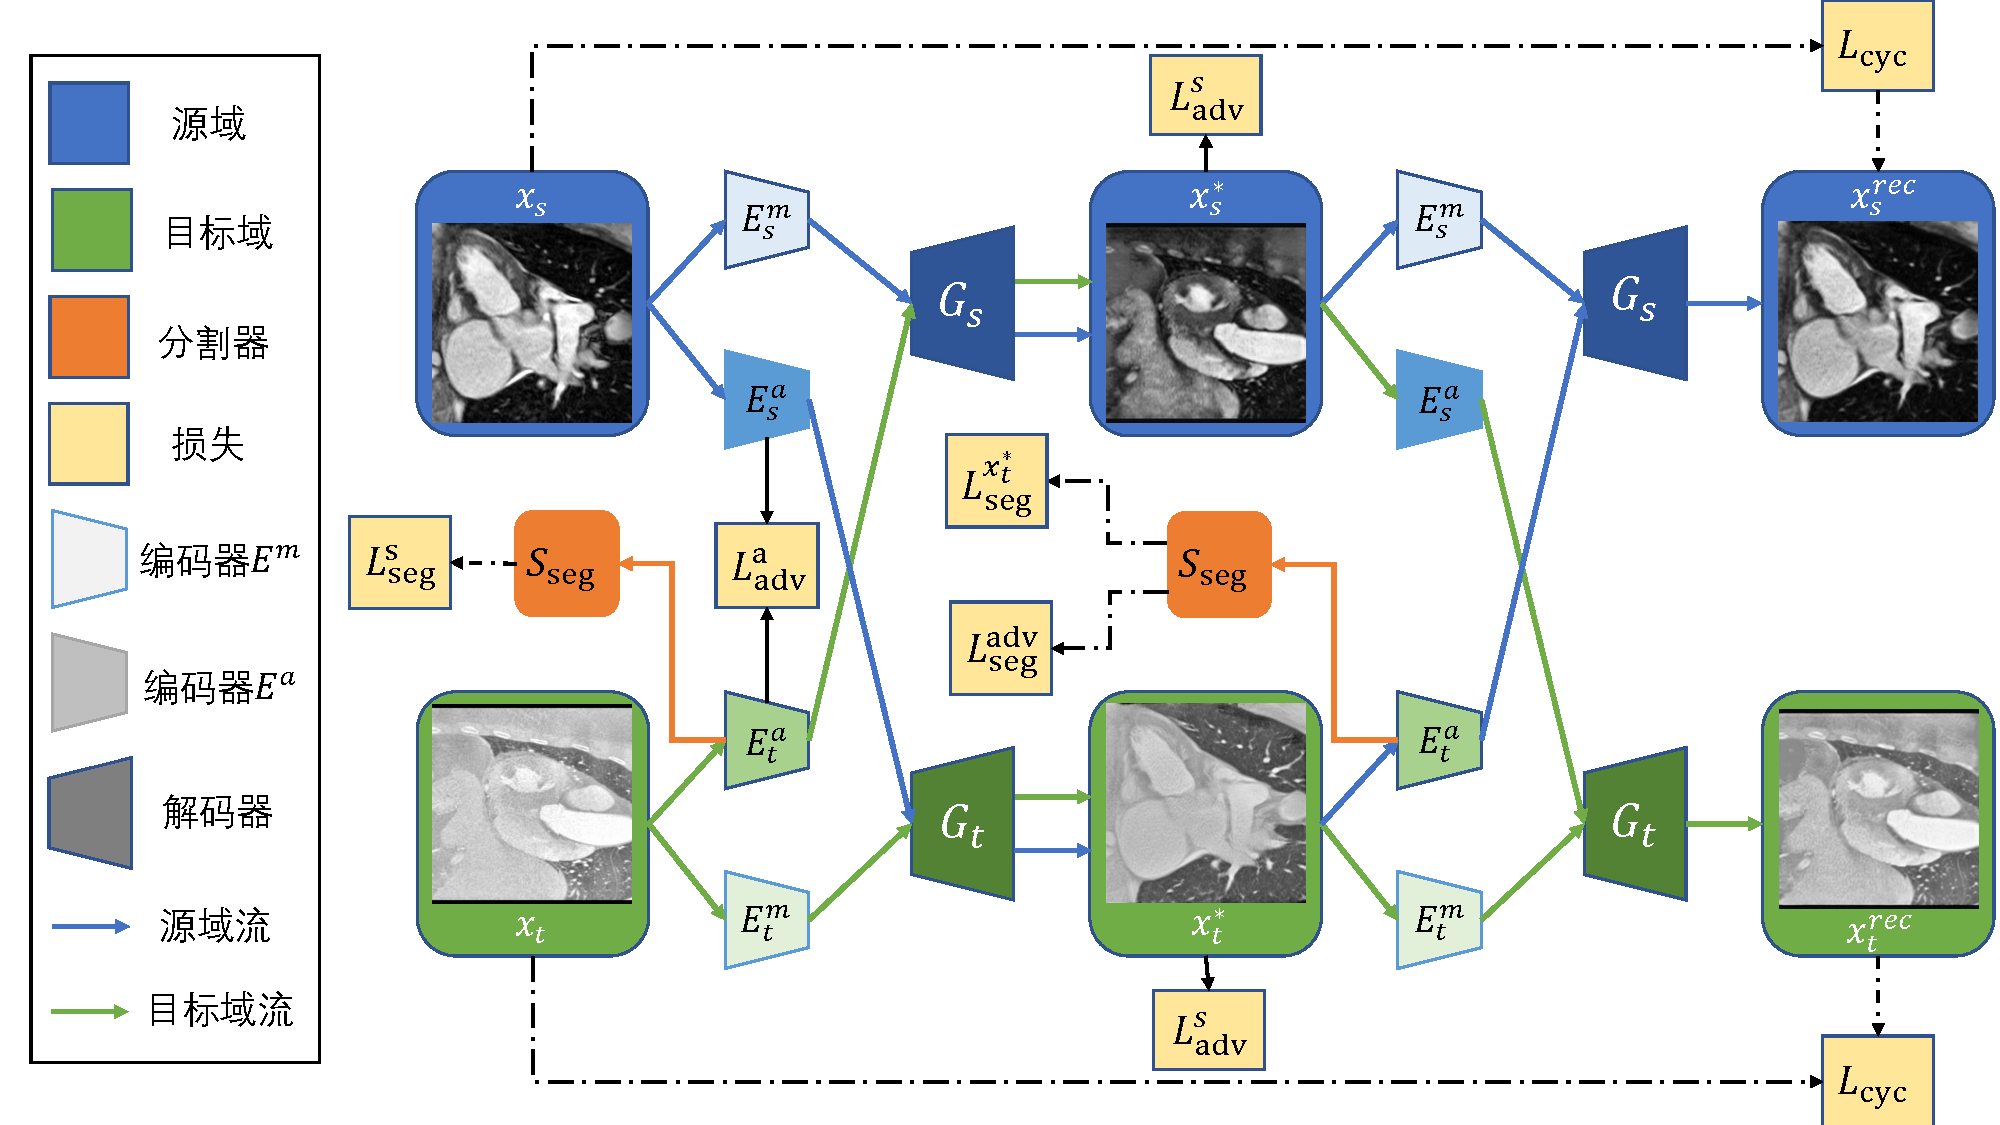
\includegraphics[width=\textwidth]{image/chap03/network structure.pdf}
        \end{figure}
}

\frame {
        \frametitle{目录}
        %\begin{multicols}{2}
        \tableofcontents[sections={<1-7>}]
}

%%
% 引言或背景
% 引言是论文正文的开端,应包括毕业论文选题的背景、目的和意义;对国内外研究现状和相关领域中已有的研究成果的简要评述;介绍本项研究工作研究设想、研究方法或实验设计、理论依据或实验基础;涉及范围和预期结果等。要求言简意赅,注意不要与摘要雷同或成为摘要的注解。
% modifier: 黄俊杰(huangjj27, 349373001dc@gmail.com)
% update date: 2017-04-15
%%

\chapter{绪论}
%定义,过去的研究和现在的研究,意义,与图像分割的不同,going deeper
\label{cha:introduction}
\section{选题背景与意义}
\label{sec:background}
% What is the problem
% why is it interesting and important
% Why is it hards, why do naive approaches fails
% why hasn't it been solved before
% what are the key components of my approach and results, also include any specific limitations,do not repeat the abstract
%contribution
随着医疗技术的进步,各种新型的医学影像设备已广泛应用在临床诊断中,其中包括计算机断层扫描(CT)、磁共振成像(MRI)、超声成像(UI)等。医学图像中含有非常有用的信息,医生可利用CT及其他医学图像来诊断患者病情,医学图像已逐渐成为临床诊断的主要依据,因此,对医学图像处理的研究具有重要意义。其中,医学图像分割是该领域的研究热点,属于语义分割的一种,图像分割将图像划分成多个解剖学意义的区域,并在此基础上可以计算相应区域的相关定量指标用于辅助临床诊断。

一般地,医学图像分割可以用集合论的术语描述\cite{liu2021review}:给定一张医学图像$I$以及相似性约束集合$C_i\ (i=1,2,\dots)$,对图像$I$的分割即得到其分划:
\begin{align}
    \bigcup_{\mathrm{x}=1}^{\mathrm{N}} R_{x}=\mathrm{I}, \quad R_{x} \cap R_{y}=\varnothing, \quad \forall x \neq y, x, y \in[1, N]
\end{align}
其中每个$R_x$中的所有像素都满足相似性约束$C_i\ (i=1,2,\dots)$,代表不同病理学意义的区域。利用传统的图像处理方法和机器学习方法来进行医学图像分割往往需要繁琐的特征工程或先验知识,而深度学习能够自动提取出复杂有效的特征,基于卷积神经网络的方法已经广泛应用在医学图像处理当中。

\begin{figure}
    \centering
    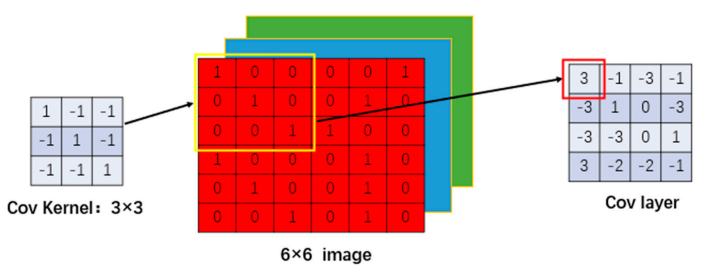
\includegraphics[width=\textwidth]{image/chap01/cnn.png}
    \caption{2D卷积神经网络卷积运算过程,图源\cite{liu2021review}}
    \label{fig:cnn}
\end{figure}
卷积神经网络已成功地应用于许多图像分类、目标检测和分割任务。假设输入图像的大小为$H\times W\times 3$,大小为$(h, w, c)$的卷积核在图像的空间维度进行滑动,在每个通道进行相应位置的卷积运算,具体的2D卷积神经网络计算过程如图\ref{fig:cnn}所示。由卷积神经网络,下采样层,激活函数组成的深层神经网络在医学图像分割中已取得了良好的效果\cite{ronneberger2015u,chen2014semantic,badrinarayanan2017segnet},其中U-Net\cite{ronneberger2015u}的使用最为广泛,对其结构的拓展仍为该领域的热门方向。

U-Net网络由一个U型网络和跳跃连接组成,如图\ref{fig:unet}。该U型网络类似一种编码器解码器的结构。编码器包含四个子模块,每个子模块包含两层卷积神经网络及用于下采样的最大池化层,对称地,解码器的四个子模块也包含两层神经网络及上采样层。同时,解码器每个子模块的输入由上个子模块的输出以及编码器中对称的子模块的输出跳跃连接组成,二者具有相同的分辨率,为的是结合网络结构低层和高层中的语义信息,帮助提取出图像中更复杂的结构,提升分割的准确率。
\begin{figure}
    \centering
    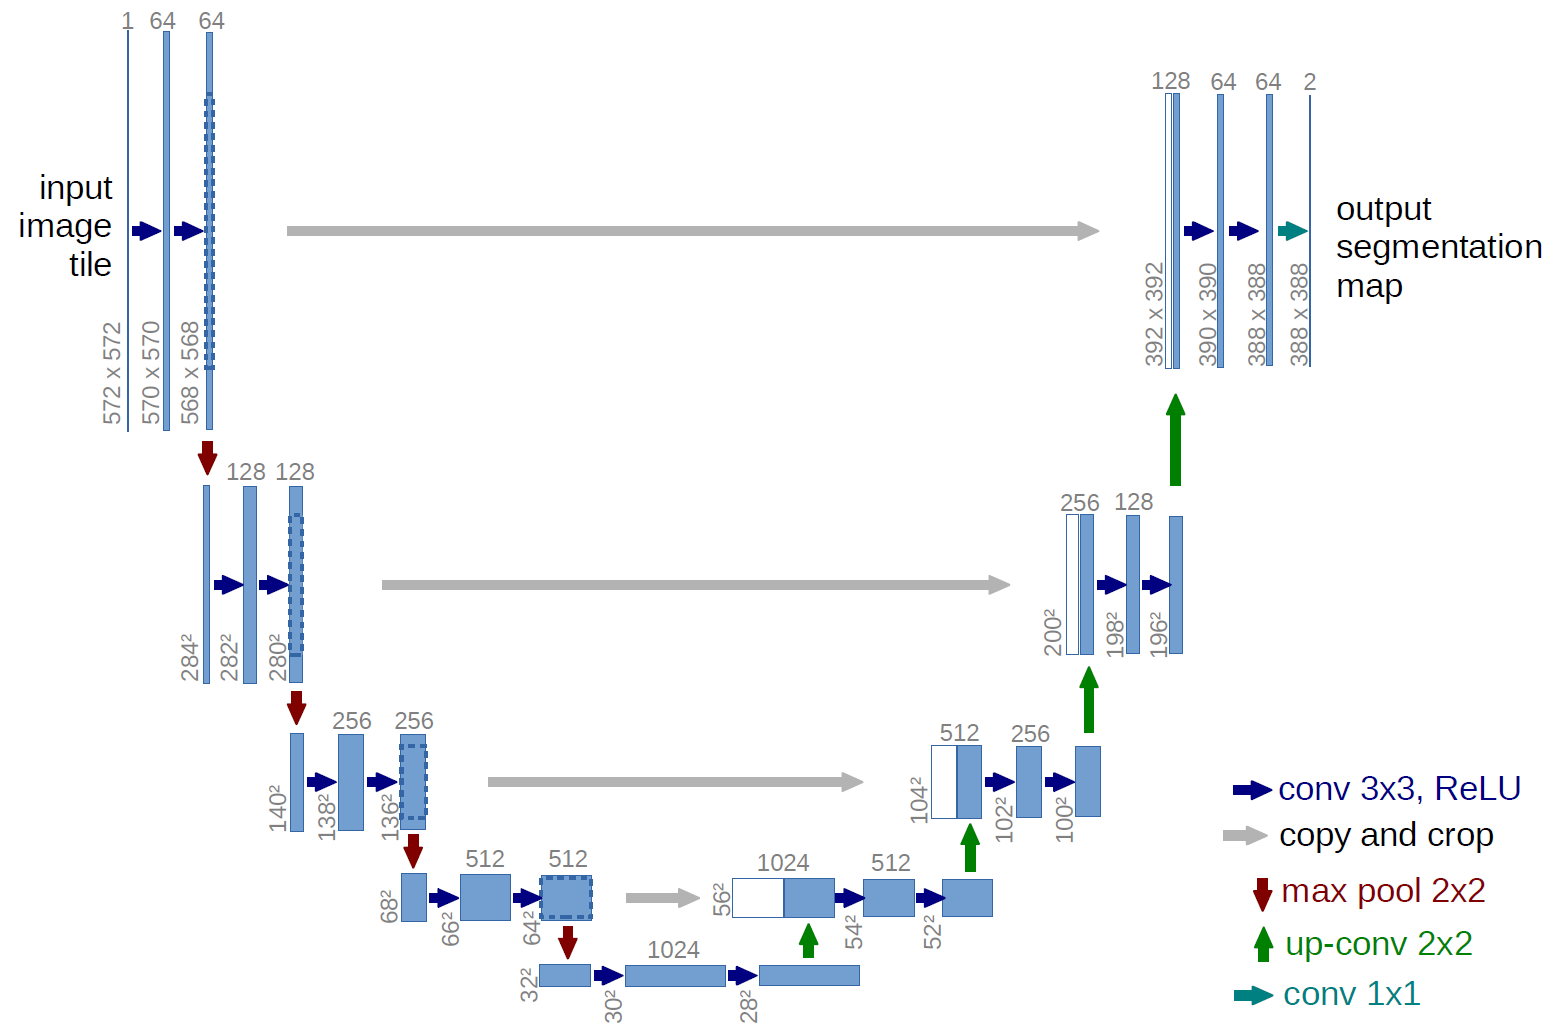
\includegraphics[width=0.8\textwidth]{image/chap01/u-net-architecture.png}
    \caption{U-Net网络结构,图源\cite{ronneberger2015u}}
    \label{fig:unet}
\end{figure}

在临床诊断中,多模态的医学图像常被用于辅助诊断,而医学图像的标注成本比较昂贵,专家标注一张完整的分割图像大约需要8小时\cite{zhuang2013challenges},解决这个问题的一种不失为有效的方法是基于学习的方法对一种模态的已有标注数据进行建模并用于另一种模态的图像分割。然而,机器学习方法通常假设训练集和测试集同属于一个数据分布,这个假设在该实际的临床场景中通常不成立,在训练集上训练好的模型在测试集上不能得到很好的泛化。先前的研究表明,测试误差会随着训练集和测试集的分布差异而增加\cite{ben2007analysis},这就是域位移问题,训练集(源域)和测试集(目标域)的分布具有一定的差异。在医学图像领域,由于各种成像模式具有不同的物理原理,异构域位移的情况更加常见和严重,如多中心,跨模态等,见图\ref{fig:hist}。在不需要目标域的带标注数据的情况下,无监督域自适应(Unsupervised Domain Adaptation,UDA)是解决由域位移带来的性能下降的一种方法。由于不需要额外的标注数据,UDA在医学图像领域中越来越受到关注。

在UDA的框架中,我们称带标注数据为源域,不带标注的数据为目标域,UDA的目的对齐源域和目标域数据的分布,一种方法是特征自适应\cite{long2017deep, sun2016deep, wu2020cf, wu2021unsupervised, dou2018pnp, tsai2018learning, vesal2021adapt},将不同模态的图像映射到一个模态不变的特征空间,另一种方法是图像自适应\cite{zhu2017unpaired},将图像从一种模态直接转换为有着相同解剖学结构的另一种模态。对于特征自适应,可以通过距离度量来显式地减小源域和目标域在特征空间上的分布差异,此外,也可以通过对抗学习来隐式地减小源域和目标域的差异。近期的研究\cite{hoffman2018cycada,chen2019synergistic}提出特征自适应和图像自适应从互补的角度来缓解域位移问题,二者有效地相结合能够改进域自适应的表现。此外,多模态的医学图像具有丰富的层次性特征,一些工作\cite{yang2019unsupervised, chartsias2019disentangled, pei2021disentangle}利用解耦表示学习来提取医学图像中的域不变特征以及域特定特征。
\begin{figure}
    \centering
    \begin{subfigure}{0.3\textwidth}
        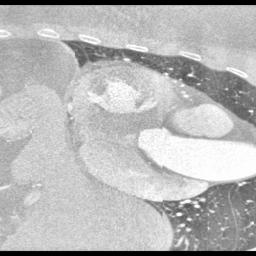
\includegraphics[width=.8\textwidth,height=.8\textwidth]{image/chap01/ct.jpeg}
        \caption{CT图}
        \label{hist:a}
    \end{subfigure}
    \hfill
    \begin{subfigure}{0.3\textwidth}
        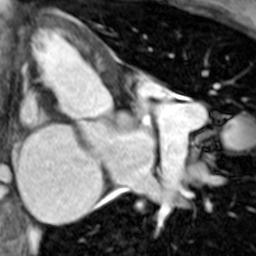
\includegraphics[width=.8\textwidth,height=.8\textwidth]{image/chap01/mr.jpeg}
        \caption{MRI图}
        \label{hist:b}
    \end{subfigure}
    \hfill
    \begin{subfigure}{0.3\textwidth}
        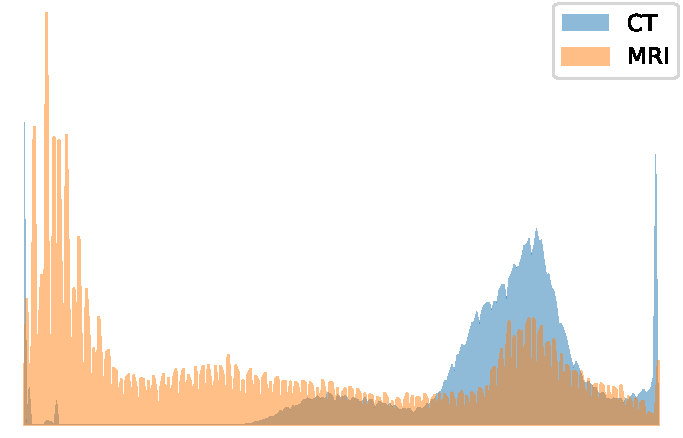
\includegraphics[width=\textwidth,height=.8\textwidth]{image/chap01/hist.pdf}
        \caption{灰度直方图}
        \label{hist:c}
    \end{subfigure}
    \caption{心脏的CT图,MRI图及其对应的灰度直方图}
    \label{fig:hist}
    \end{figure}


\section{本文方法概述}
\label{sec:contributions}
本文提出了一个新的UDA框架用于跨模态医学图像分割。该框架基于解耦表示学习来提取出不同模态的心脏图像的模态特征以及解剖学特征,结合图像自适应和特征自适应,进而利用不同模态的医学图像之间具有相似的解剖学特征来实现跨模态的医学图像分割。主要贡献如下:
\begin{itemize}
    \item 利用解耦表示学习提取出跨模态医学图像的模态特征和解剖学特征,进而实现非成对跨模态图像之间的转换。
    \item 在CT-MRI多模态心脏数据集进行相关实验,验证了方法的有效性。
\end{itemize}

\newpage
\section{本文的论文结构与章节安排}
\label{sec:arrangement}

本文共分为六章,各章节内容安排如下:

第一章绪论。简单说明了本文章的选题背景与意义。

第二章为本领域的相关工作。

第三章为本文方法的详细介绍。

第四章为实验与结果。

第五章为总结与展望。


% \chapter{相关工作}

\label{cha:related work}


\section{基于无监督域自适应的医学图像分割}
最近,UDA方法已广泛应用在医学图像领域的研究中。现有的UDA方法通常从三个角度对齐源域和目标域的分布。第一类是特征自适应,通常是为了提取域不变特征,最小化域之间的特征分布差异。第二类是图像自适应,通过基于生成对抗网络的图像到图像转换实现跨域图像外观和风格的转变。第三类关注的是二者的结合。
\subsection{特征自适应}
传统的UDA方法大多通过距离度量来显式地减小源域和目标域的特征空间的分布差异。其中,MMD\cite{long2017deep}是一种常用的距离度量。相应的一些扩展利用了特征分布的一些统计量,如协方差\cite{sun2016deep},特征函数\cite{wu2020cf}来进行特征对齐。但由于用于图像分割的特征空间应该包括各种视觉线索,如外观,可能过于复杂和高维,显式的距离度量如KL散度,Wasserstein距离在考虑批量数据的情况下通常没有解析式,而使用其他的一些度量如MMD,减小分布差异效果不明显,而CFD\cite{wu2020cf}在高维数据空间进行反向梯度传播会造成不可忽视的误差\cite{wu2021unsupervised}。因此,另外一种主流的用于图像分割的域自适应方法是对抗学习,一些工作通过对抗学习隐式地对齐特征空间,从而学习到域不变的特征表示。对于存在严重域位移问题的跨模态分割,\citeauthor{dou2018pnp}\cite{dou2018pnp}通过微调具体的特征层并对监督特征采用对抗损失学习。\citeauthor{tsai2018learning}\cite{tsai2018learning}过对齐输出空间来整合空间和几何结构信息。\citeauthor{wang2019boundary}\cite{wang2019boundary}提出了一种方法对眼底图像的熵和边界进行对抗自适应。\citeauthor{vesal2021adapt}\cite{vesal2021adapt}通过对齐点云来对齐形状特征。

\subsection{图像自适应}
近年来一些图像到图像转换的方法如CycleGAN\cite{zhu2017unpaired}利用生成对抗网络来把源域的图像转换为与目标域风格类似的图像。然后,这些生成的图像继承了源域图像的分割图,可以用于目标域分割网络的监督学习。\citeauthor{zhang2018translating}\cite{zhang2018translating}利用循环和形状一致性对抗网络进行多模态大脑MRI分割。在\citeauthor{liu2019unpaired}\cite{liu2019unpaired}中,作者结合基于注意力的神经网络生成目标域图像。\citeauthor{yang2019unsupervised}\cite{yang2019unsupervised}启发于解耦表示的思想,训练变分自编码器将图像模态特征和内容特征进行解耦,从而用来生成不同域的图像。

\subsection{特征和图像自适应}
近年来,一些研究提出将特征自适应和图像自适应结合起来,能更好地减轻域位移的影响\cite{hoffman2018cycada,chen2019synergistic}。CyCADA\cite{hoffman2018cycada}将UDA作为一种风格迁移方法减小源域和目标域之间的外观差距,同时独立地对齐两个域的潜在特征空间。\citeauthor{chen2019synergistic}\cite{chen2019synergistic}提出了SIFA框架,不同于\cite{hoffman2018cycada},其协同利用特征自适应和图像自适应成统一的网络,从互补的角度来对齐心脏图像MRI和CT两种模态的分布。他们还扩展SIFA为Bidirectional-SIFA\cite{chen2020unsupervised},添加深度监督特征的对齐,以及从双向的角度(MRI$\leftrightarrow$ CT)来探索领域自适应在多模态医学图像分割的应用。\citeauthor{han2021deep}\cite{han2021deep}提出了一个对称结构的域自适应网络。\citeauthor{tomar2021self}\cite{tomar2021self}利用自注意空间自适应标准化的结构来使得网络关注医学图像中具有解剖学意义的区域。\citeauthor{ye2021unsupervised}\cite{ye2021unsupervised}利用对比学习和原型相似度比较来显式地对齐源域和生成图像的特征。

\section{解耦表示学习}
对图像特征进行解耦已广泛应用于图像转换和风格迁移等计算机视觉应用任务中\cite{DRIT, DRIT_plus}。InfoGAN\cite{chen2016infogan}将特征解耦成可解释的潜变量与噪声,同时最大化生成数据与潜变量之间的互信息,使得生成数据与潜变量更相关。\citeauthor{yang2019unsupervised}\cite{yang2019unsupervised}通过训练变分自编码器将图像特征进行解耦,得到8维的风格特征以及高维表示的内容特征,利用自适应实例归一化(Adaptive Instance Normalization,AdaIN)和风格特征对内容特征进行仿射变换,进而实现不同域之间图像的风格迁移。最近的研究也开始将解耦表示学习用于医学影像分析当中\cite{chartsias2019disentangled,chen2019robust,pei2021disentangle}。\citeauthor{pei2021disentangle}\cite{pei2021disentangle}利用自注意力机制和归零损失函数来进一步对医学图像特征进行解耦,进而完成跨模态的医学图像分割。


% \chapter{方法}
\label{cha:method}
记来自源域的带标注数据集为$\mathbb{D}_s = \{x^s_i, y_i^s\}_{i=1}^{m_s}$,其中$x_i^s\in \mathbb{R}^{w\times h \times 3},y_i^s\in \mathbb{R}^{w\times h\times c}$,$c$是图像中具有不同语义结构的数目,$m_s$表示源域数据集的大小。记来自目标域的无标注数据集$\mathbb{D}_t=\{x_i^t\}_{i=1}^{m_t}$,$m_t$表示目标域数据集的大小。我们旨在利用带标注的源域数据集来对目标域的医学图像进行语义分割。这篇文章将图像的特征进行解耦,从而学习到两个域的解剖学特征和模态特征,文章提出的框架如图\ref{fig:network}所示。对于每个模态的图像,首先利用编码器得到对应域的解剖学特征以及模态特征,然后交换各自的模态特征,将相应的解剖学特征和模态特征输入到解码器得到另一个模态的图像。参考CycleGAN,重复编码解码的操作对原图像进行重构。\footnote{开源代码:\url{https://github.com/Lawliet-Xie/undergraduate-thesis}}

\section{利用解耦表示来进行图像自适应}
不同模态的医学图像通常具有相似的解剖学结构,即域不变特征,二者的差异往往来自于其不同的模态特征,即域特定的特征。将这些特征进行解耦,进而实现跨模态图像之间的转换。如图所示,编码器$E_d^{anatomy}$和$E_d^{modality}$(下文将解剖学特征anatomy简记为a,模态特征modality简记为m)分别提取图像的解剖学特征以及模态特征,数学形式的表达即$z_d^{c} = E^c_d{x^d}$,其中$c\in \{a,m\}, d\in \{s,t\}$。为了实现解耦表示,常用的方法是通过权重共享将跨模态图像的解剖学特征映射到同一个空间,然而,权重共享很难保证编码出相同的解剖学特征表示。这里引入判别器$D_a$来隐式地对齐跨域的域不变特征,其对抗损失为
\begin{align}
\begin{aligned}L_{\mathrm{adv}}^{\text {a }} &=\mathbb{E}_{x_s}\left[\frac{1}{2} \log D_a\left(z_s^a\right)+\frac{1}{2} \log \left(1-D_a\left(z_s^a\right)\right)\right] \\&+\mathbb{E}_{x_t}\left[\frac{1}{2} \log D_a\left(z_t^a\right)+\frac{1}{2} \log \left(1-D_a\left(z_t^a\right)\right)\right].\end{aligned}
\end{align}
得到解耦表示后,两个域特定的解码器,记为$G_s$,$G_t$,用于生成两个模态的伪图。如图所示,$G_s$可以结合源域图像$x_s$的模态特征和目标域图像$x_t$的解剖学特征来生产伪图$x_s^*=G_s(z_s^{m},z_t^{a})$,同理,我们可以利用$D_t$得到$x_t^*=G_t(z_t^{m},z_s^{a})$。启发于CycleGAN,重复该过程对原图像进行重构,得到$x_s^{\mathrm{rec}}$和$x_t^{\mathrm{rec}}$,即$x_s^{rec} = G_s(E_s^{m}(x_s^*),E_t^{a}(x_t^*)), x_t^{rec} = G_t(E_t^{m}(x_t^*),E_s^{a}(x_s^*))$。这些重构的图像应与原图像一致,故有循环一致性损失(cycle consistency loss):
\begin{align}
\mathcal{L}_{cyc} = \mathbb{E}_{(x_s,x_t)\in P(\mathbb{D}_s,\mathbb{D}_t)}\|x_s^{rec}-x_s\|_1 + \mathbb{E}_{(x_s,x_t)\in P(\mathbb{D}_s,\mathbb{D}_t)}\|x_t^{rec}-x_t\|_1 .
\end{align}
其中$\|\cdot \|_1$代表L1范数。

此外,为了使得伪图$x_s^*$和$x_t^*$接近于真实的图像,引入两个判别器$D_s$和$D_t$,用于对抗学习。基于生成对抗网络的思想,判别器$D_s$能够分别出$x_s$是真图,而$x_s^*$是伪图,同时以上的由编码器解码器组成的生成器结构能够生成出足够真实的样本来干扰判别器,$D_t$同理。故目标函数为:
\begin{align}
&\min_{(E_s^{a},E_t^{m},G_t)}\max_{D_t} \mathcal{L}_{adv}^t= \mathbb{E}_{x_t\in P(\mathbb{D}_t)}[\log D_t(x_t)] + \mathbb{E}_{(x_s,x_t)\in P(\mathbb{D}_s,\mathbb{D}_t)}[\log (1-D_t(x_t^*))],\\
&\min_{(E_t^{a},E_s^{m},G_s)}\max_{D_s} \mathcal{L}_{adv}^s= \mathbb{E}_{x_s\in P(\mathbb{D}_s)}[\log D_s(x_s)] + \mathbb{E}_{(x_s,x_t)\in P(\mathbb{D}_s,\mathbb{D}_t)}[\log (1-D_s(x_s^*))].
\end{align}


\begin{figure}
    \centering
    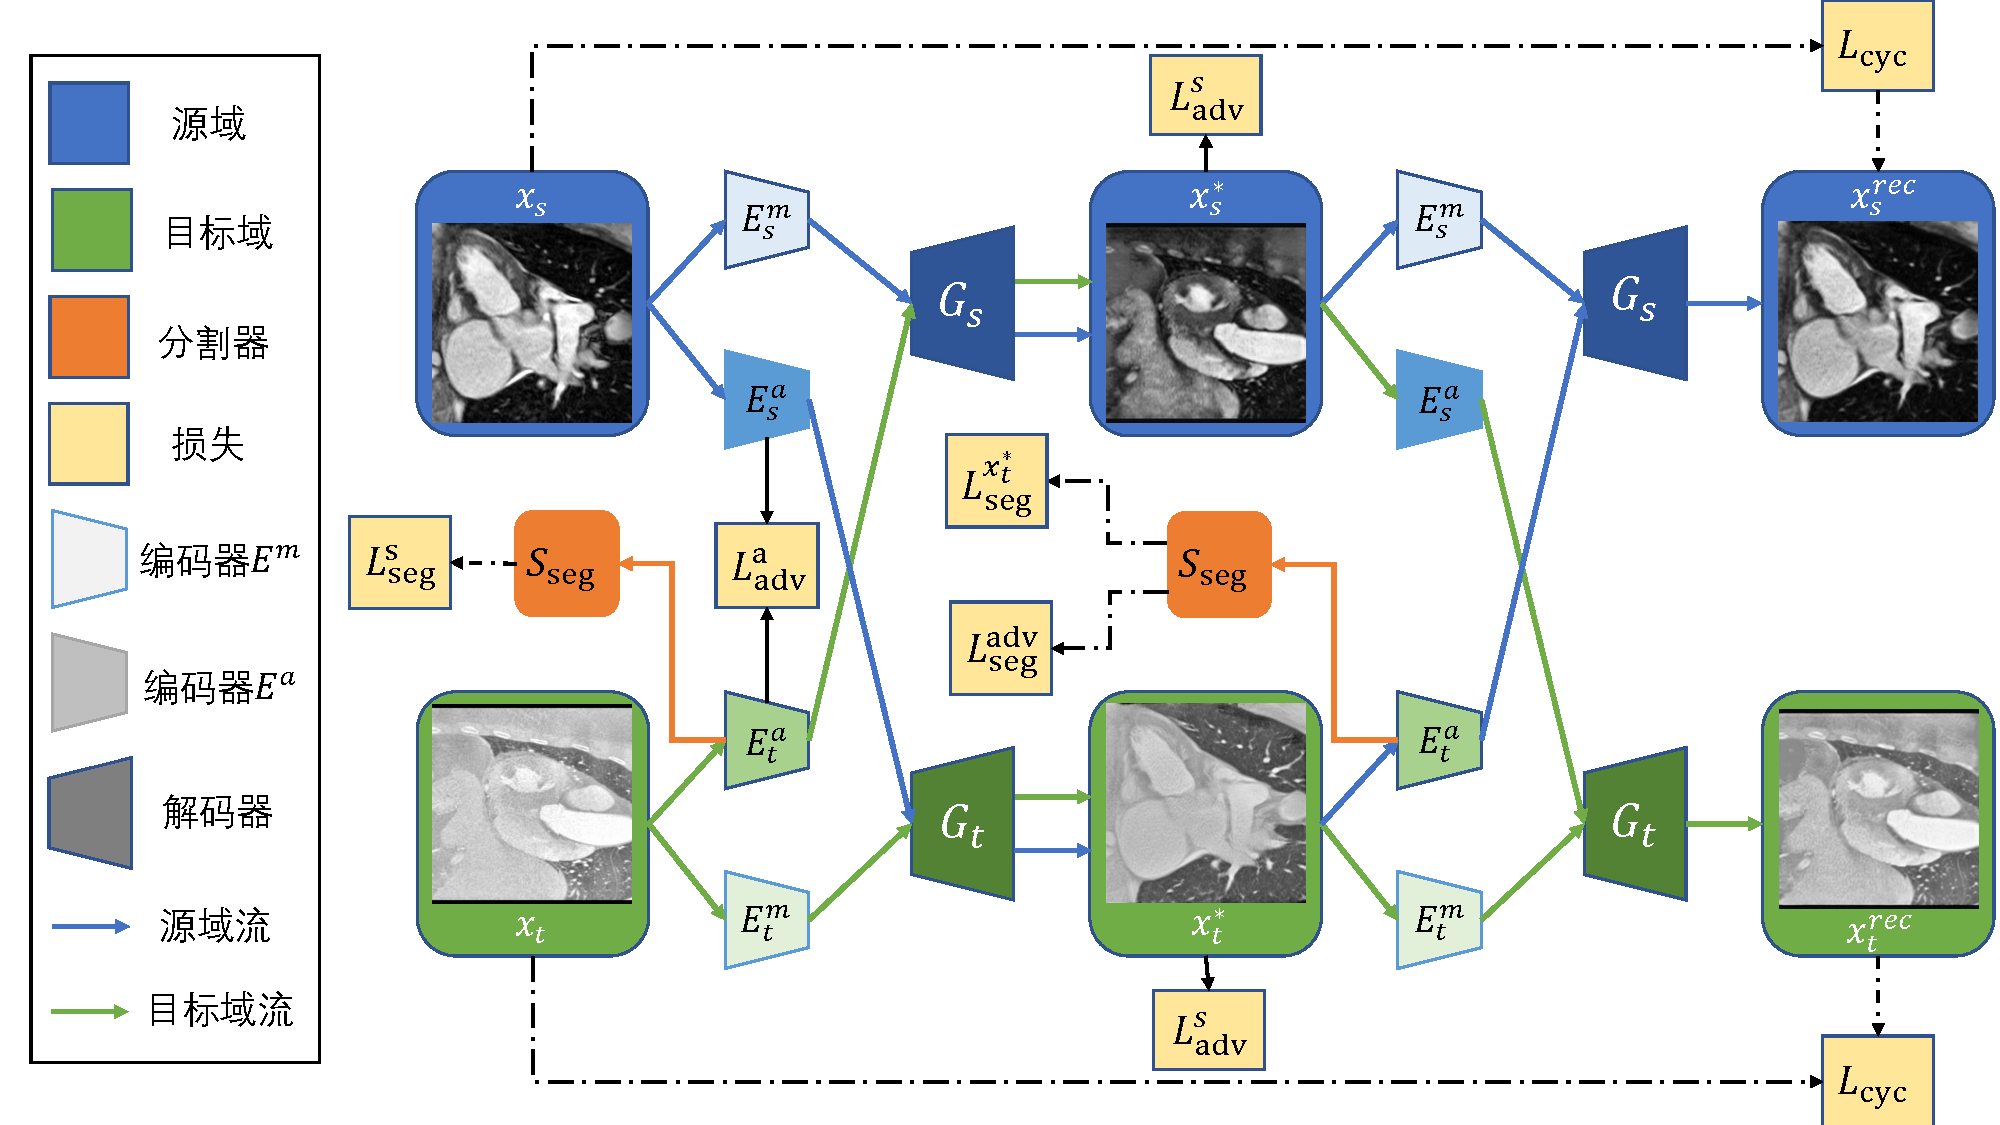
\includegraphics[width=\textwidth]{image/chap03/network structure.pdf}
    \caption{整体网络结构}
    \label{fig:network}
\end{figure}

\section{框架各组成成分的网络结构}
\subsection{编码解剖学特征}
解耦解剖学特征的编码器由卷积神经网络组成,将2D的医学图像映射到其空间表示,即$E^a:x\rightarrow z^a$,其中$z^a\in \mathbb{R}^{w\times h\times k}$,k表示所需要的解剖学特征数。编码器整体采用类似U-Net\cite{ronneberger2015u}的网络结构,如图\ref{fig:enc_anatomy}所示,包含了下采样,上采样以及跳跃连接,能够有效地融合重要的局部和非局部信息,提取出丰富的语义信息,得到特征中的每个通道表示心脏中一些具有解剖学意义的子结构。
\begin{figure}
    \centering
    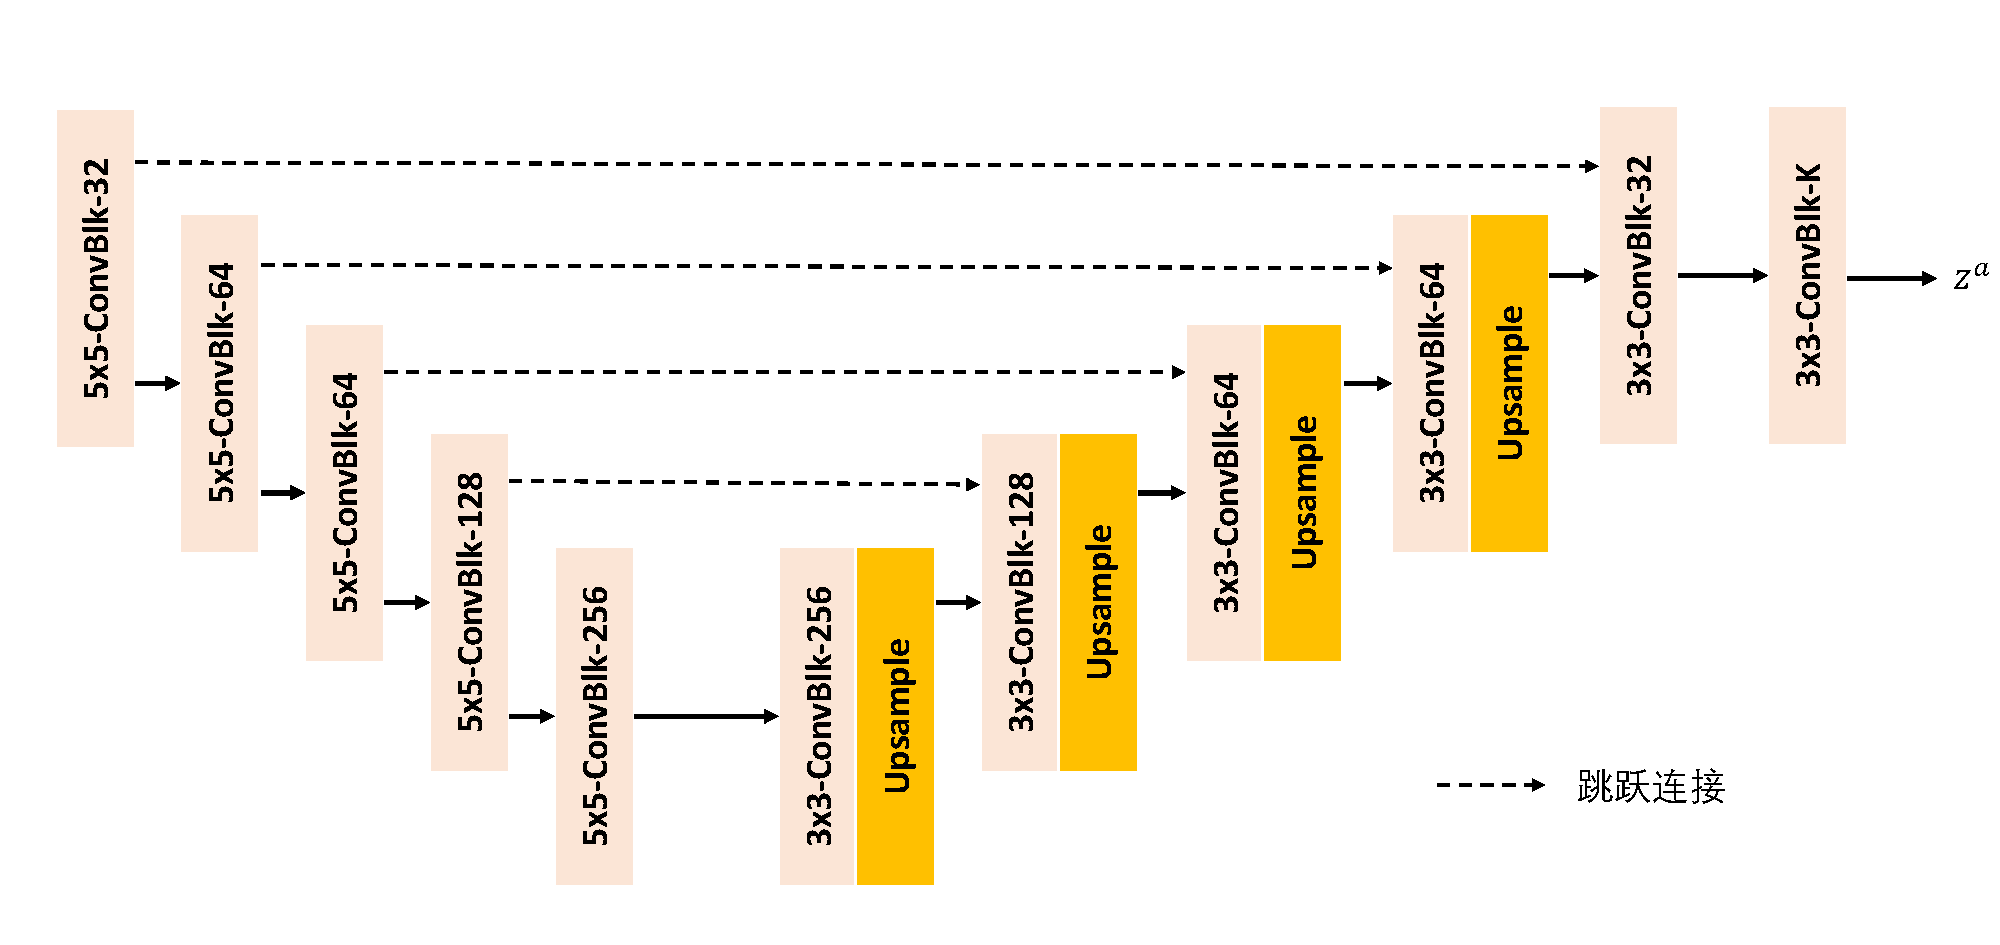
\includegraphics[width=\textwidth]{image/chap03/encoder_anatomy.pdf}
    \caption{解剖学特征编码器}
    \label{fig:enc_anatomy}
\end{figure}
\subsection{编码模态特征}
编码器$E^m$为了学习到医学图像模态特征$z^m$的后验分布$q(z^m|x)$,采用变分自编码器\cite{kingma2013auto}(Variational Autoencoder, VAE)。简单地说,VAE学习一个低维的潜空间,该特征空间中的潜表示能够匹配一个先验分布$p(z)=\mathcal{N}(\bold{0},I)$,从风格迁移和解耦表示的角度来说,从该空间中进行模态的采样,能够生成各种模态的图像,整体结构如图\ref{fig:enc_modality}所示。
\begin{figure}
    \centering
    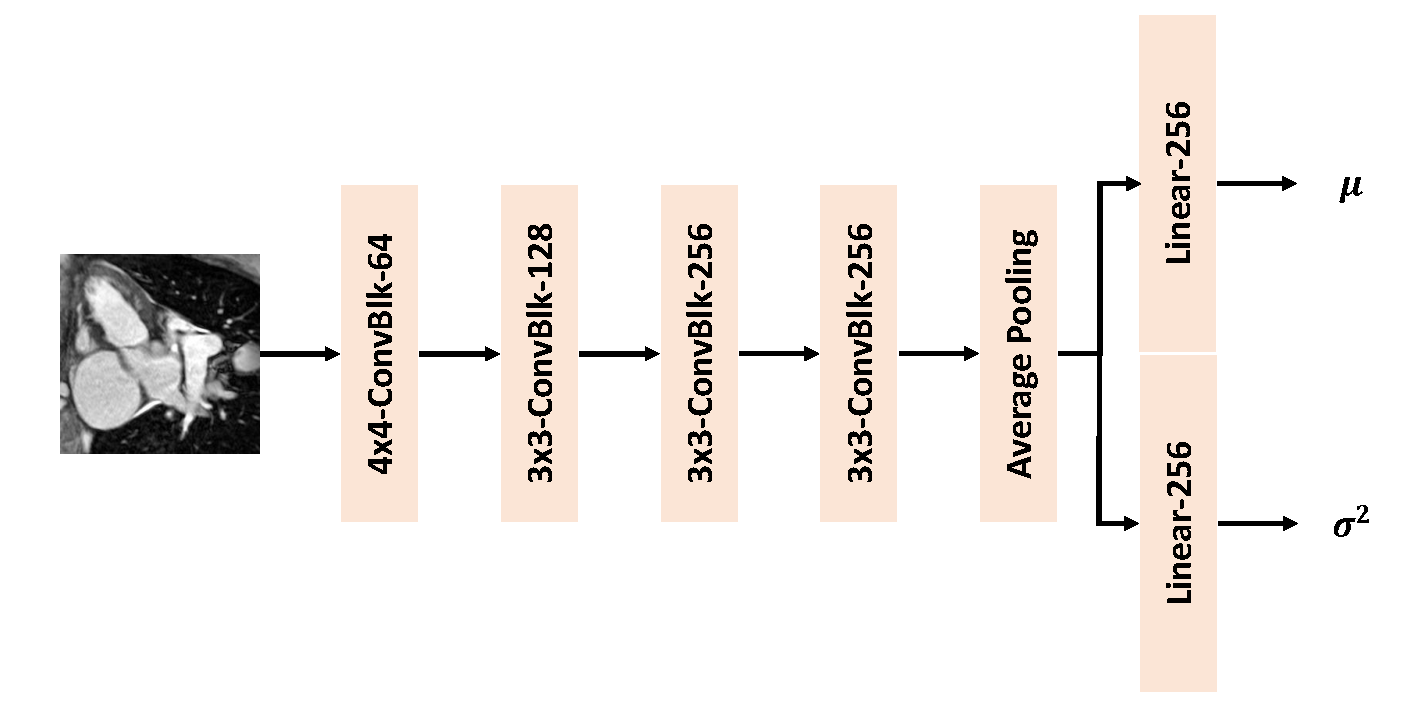
\includegraphics[width=\textwidth]{image/chap03/encoder_modality.pdf}
    \caption{模态特征编码器}
    \label{fig:enc_modality}
\end{figure}

\subsection{解码器}
解码器$G$以模态特征和解剖学特征作为输入,用于进行图像的生成与重构。SPADE\cite{park2019semantic}(Spatially Adaptive Denormalization)是一种能有效利用语义信息以及风格信息进行图像生成的一种结构。与普通的卷积神经网络对比,其通过空间自适应归一化来更好地保留语义信息,具体公式如下:
\begin{align}
    \begin{split}
    \hat{x}_{c,i,j}(z^a) &=\gamma_{c,i,j}(z^a) * \frac{z^m_{c,i,j}-\mu_{c}}{\sigma_{c}}+\beta_{c,i,j}(z^a) \\
    \mu_{c} &=\frac{1}{H W} \sum_{i, j} z^m_{c,i,j},\quad \sigma_{c}^{2}=\frac{1}{H W} \sum_{i, j}\left(z^m_{c,i,j}-\mu_{c}\right)^{2}
    \end{split}
\end{align}
在该模块中,解剖学特征$z^a$被映射到一个嵌入空间来产生仿射变换的参数$\gamma$和$\beta$,不同于AdaIN等其他条件归一化方法,SPADE产生的$\gamma$和$\beta$包含了空间和相应的语义信息,接着利用$\gamma$和$\beta$对已经实例归一化的模态特征$z^m$来实现多模态的图像生成\cite{park2019semantic},如图\ref{fig:spade}所示。解码器(图\ref{fig:decoder})由多个SPADE块组成,能够充分融合解剖学特征和模态特征来进行伪图的生成以及原图的重建。
\begin{figure}
    \centering
    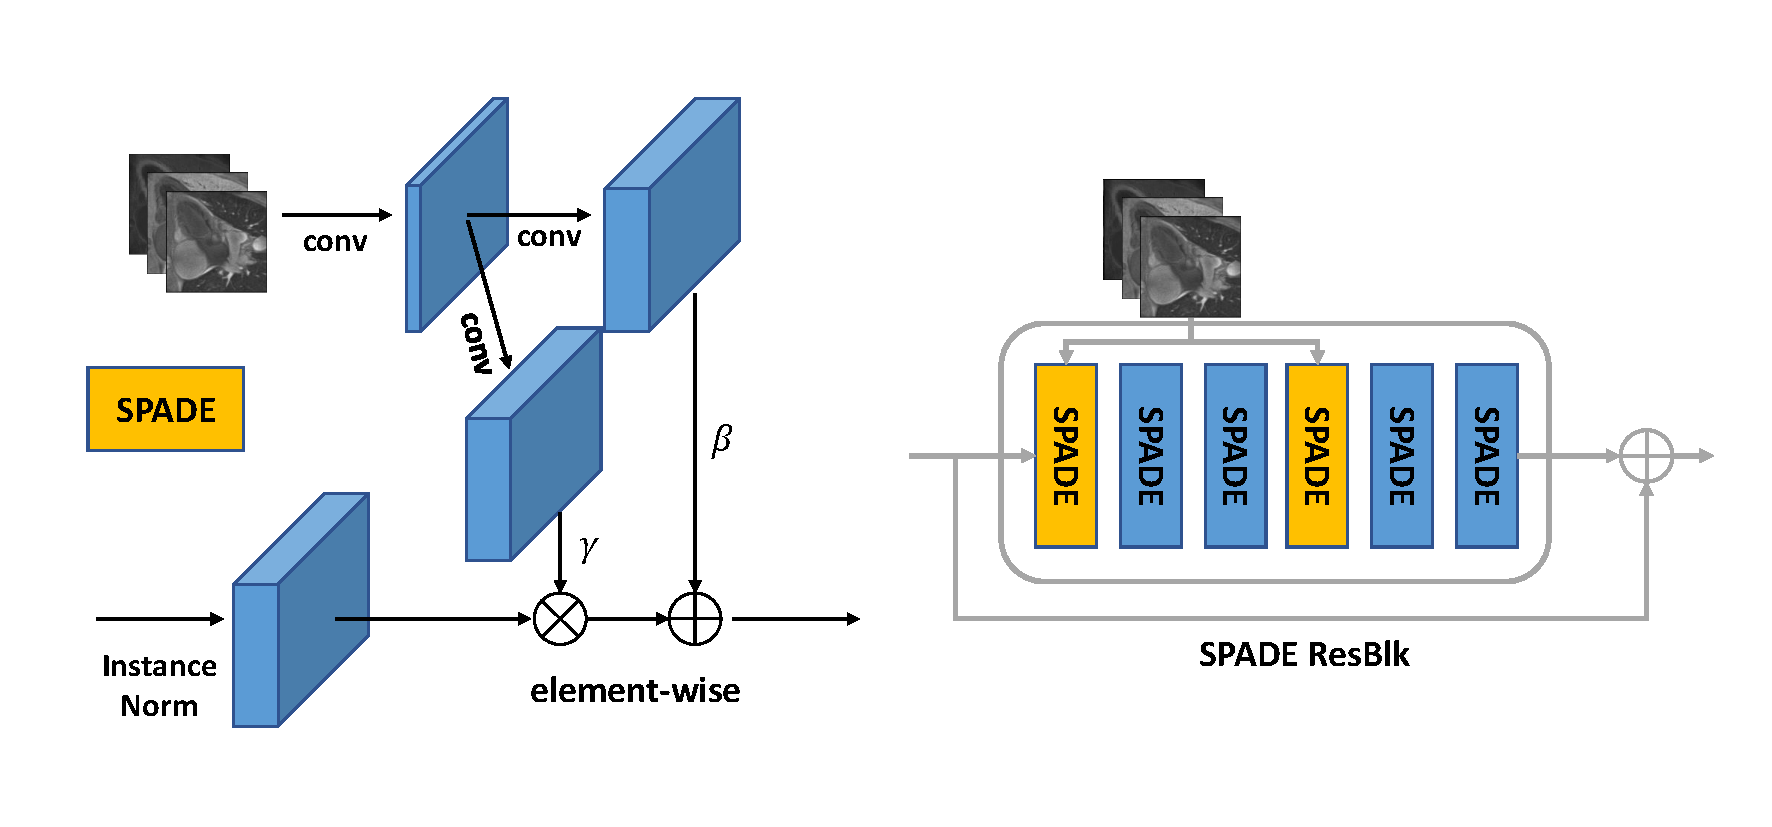
\includegraphics[width=\textwidth]{image/chap03/SPADE.pdf}
    \caption{SPADE网络结构}
    \label{fig:spade}
\end{figure}
\begin{figure}
    \centering
    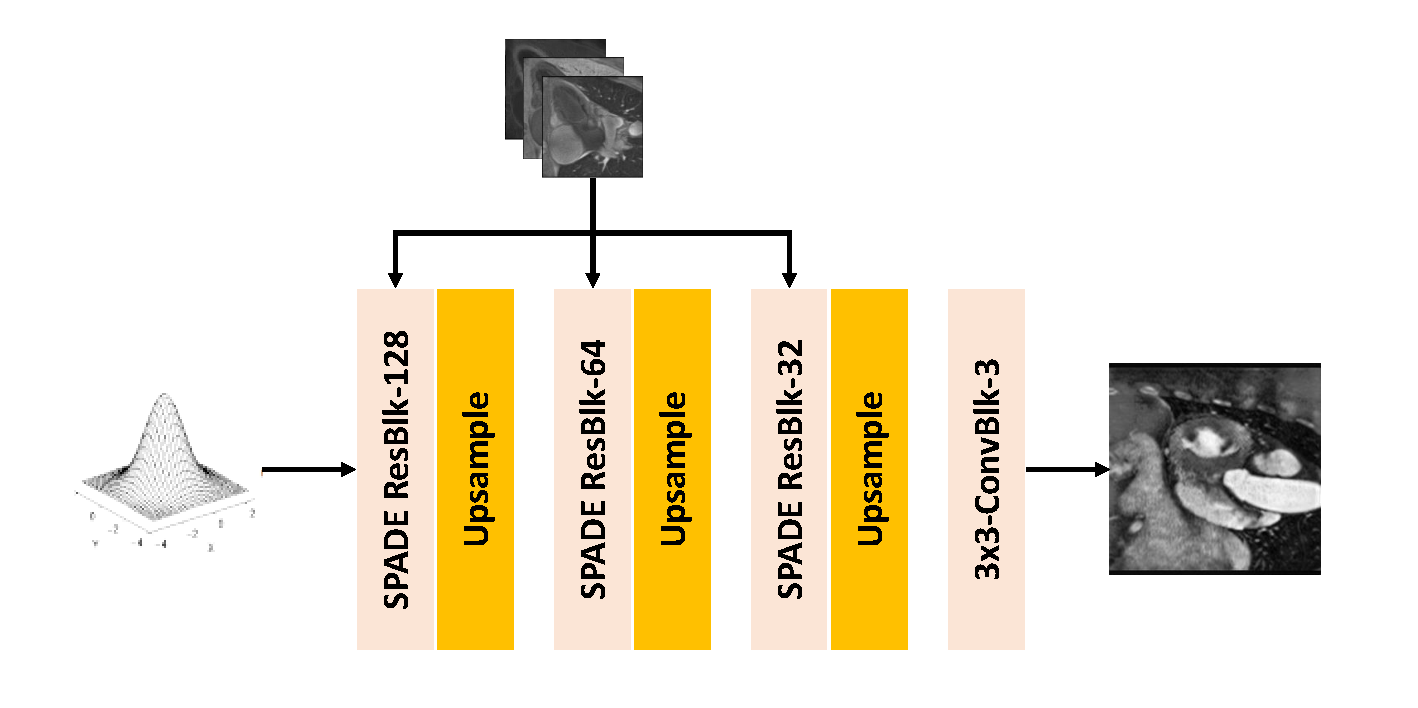
\includegraphics[width=\textwidth]{image/chap03/decoder.pdf}
    \caption{由SPADE ResBlock组成的解码器结构}
    \label{fig:decoder}
\end{figure}

\subsection{分割器}
解剖学特征已经包含了医学图像中丰富的语义信息,在此基础上增加一层卷积神经网络$S_{\mathrm{seg}}$来完成语义分割。由于源域图像带标注$y_s$,生成的伪图$x_t^*$与$x_s$共享相似的解剖学特征$z_s^a$,故$S_{\mathrm{seg}}$对二者的分割预测$\hat{y}_{t^*}$和$\hat{y}_s$能够与$y_s$进行监督学习,有如下损失:
\begin{align}
    \mathcal{L}_{\text {seg }}^{x_s}=\mathcal{H}\left(y_{s}, \hat{y}_{s}\right)+\alpha \cdot \operatorname{Dice}\left(y_{s}, \hat{y}_{s}\right),\\
    \mathcal{L}_{\text {seg }}^{x_t^*}=\mathcal{H}\left(y_{s}, \hat{y}_{t^*}\right)+\alpha \cdot \operatorname{Dice}\left(y_{s}, \hat{y}_{t^*}\right).
\end{align}
其中$H$为交叉熵损失,$\operatorname{Dice}$损失用于衡量语义分割效果,具体计算公式见附录,$\alpha$为超参数。总的分割损失可表示为$\mathcal{L}_{\mathrm{seg}} = \mathcal{L}_{\text {seg }}^{x_s} + \mathcal{L}_{\text {seg }}^{x_t^*}.$
此外,引入判别器$D_{\mathrm{seg}}$,进一步从语义空间上缩小源域和目标域图像的分布差异,
\begin{align}
    \begin{aligned}\min _{\left(E_{t}^a, S_{\text {seg }}\right)} \max _{D_{\mathrm{seg}}} \mathcal{L}_{a d v}^{\operatorname{seg}}&=\mathbb{E}_{x_{t}^{*}}\left[\log D^{\mathrm{seg }}\left(S_{\text {seg }}\left(E_{t}^a\left(x_{t}^{*}\right)\right)\right)\right] \\&+\mathbb{E}_{x_{t} }\left[\log \left(1-D_{\mathrm{seg}}\left(S_{\text {seg }}\left(E_{t}^a\left(x_{t}\right)\right)\right)\right)\right] .\end{aligned}
\end{align}

\section{其他损失函数}
\begin{itemize}
    \item 正交损失\\对得到的解剖学特征进行正交性约束,使得每个通道能学习到不同病理意义的子结构,减少特征的冗余性,更好地解耦解剖学特征和模态特征。
    \begin{align}
        \mathcal{L}_{\text {ortho}}=\mathbb{E}_{x_s}\left[\left\|E^a_s(x_s) E^a_s(x_s)^T-I\right\|_{F}\right] + \mathbb{E}_{x_t}\left[\left\|E^a_t(x_t) E^a_t(x_t)^T-I\right\|_{F}\right].
    \end{align}
    其中$I$是单位矩阵,$\|\cdot \|_F$代表Frobenius范数。
    \item KL散度损失\\该损失函数目的是使模态表示$q(z^m|x)=\mathcal{N}(\mu(x), \sigma(x)^2)$与先验高斯分布$p(z)=\mathcal{N}(\bold{0},I)$一致,从图像生成的角度,我们从该先验高斯分布中随机采样,能得到不同模态的图像。
    \begin{align}
        \begin{aligned}\mathcal{L}_{\mathrm{KL}}&=\mathcal{D}_{\mathrm{KL}}(q(z^m|x)\|p(z))\\&=-\int{q(z^m|x)\log\frac{q(z^m|x)}{p(z)}dz}\\&=\frac{1}{2}\sum_{j=1}^d(\sigma_j+u_j^2-\log \sigma_j-1).\end{aligned}
    \end{align}
    \item 重构损失\\除了交叉循环重构损失,以$E_s^a$和$E_s^m$为输入,进入解码器$G_s$理应能重构出原来的图像$x_s$,对于目标域图像$x_t$同理,即如下重构损失:
    \begin{align}
        \mathcal{L}_{\mathrm{id}} = \mathbb{E}_{x_s}[\|G_s(E_s^a(x_s),E_s^m(x_s))-x_s\|_1] + \mathbb{E}_{x_t}[\|G_t(E_t^a(x_t),E_s^m(x_t))-x_t\|_1].
    \end{align}
\end{itemize}
结合以上提到的损失函数,总的目标函数为
\begin{align}
    \begin{aligned}
    \mathcal{L} &= \lambda_1\mathcal{L}_{adv}^a +\lambda_2\mathcal{L}_{cyc} +\lambda_3\mathcal{L}_{adv}^s +\lambda_4\mathcal{L}_{adv}^t \\
    &+\lambda_5\mathcal{L}_{\mathrm{seg}} +\lambda_6\mathcal{L}_{adv}^{\mathrm{seg}} +\lambda_7\mathcal{L}_{\mathrm{ortho}} +\lambda_8\mathcal{L}_{\mathcal{\mathrm{KL}}} + \lambda_9\mathcal{L}_{id}.
    \end{aligned}
    \label{eq:loss}
\end{align}
其中,$\lambda_1,\lambda_2,\lambda_3,\lambda_4,\lambda_5,\lambda_6,\lambda_7,\lambda_8,\lambda_9$为超参数,用于平衡各个模块的重要性。第一项损失旨在使得源域和目标域图像能够提取到域不变特征,第二项和最后一项损失旨在重构回原来的图像,第三第四项损失旨在生成足够真实的伪图从而能够干扰判别器,第五项为利用监督学习进行语义分割产生的损失,其余项的提出是为了促进不同模态图像之间域自适应,缓解域位移问题。

\begin{figure}
    \centering
    \begin{subfigure}{0.45\textwidth}
        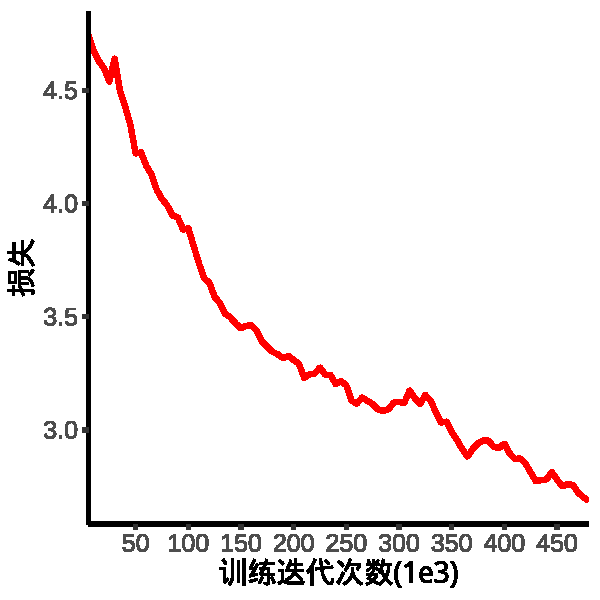
\includegraphics[width=\textwidth,height=\textwidth]{image/chap03/gen_loss.pdf}
        \caption{生成器训练损失}
        \label{fig:gen_loss}
    \end{subfigure}
    \hfill
    \begin{subfigure}{0.45\textwidth}
        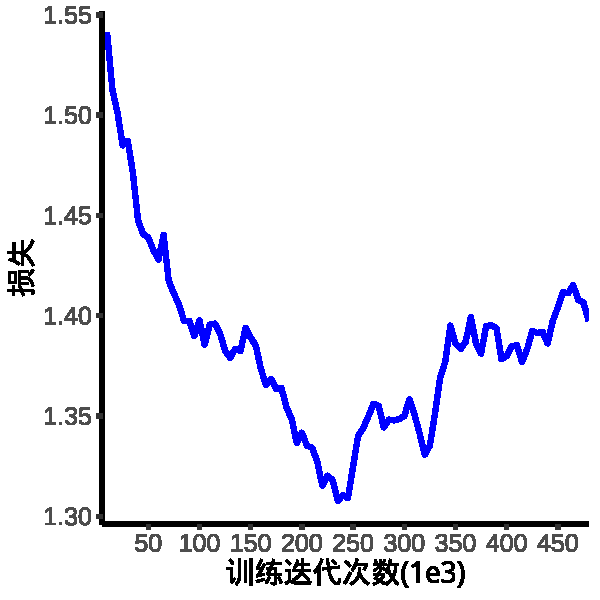
\includegraphics[width=\textwidth,height=\textwidth]{image/chap03/dis_loss.pdf}
        \caption{判别器训练损失}
        \label{fig:dis_loss}
    \end{subfigure}
    \caption{在MMWHS数据集上进行训练的损失}
    \label{fig:loss}
    \end{figure}

\section{实现细节}
这一小节我们补充训练过程中各种参数的设定以及相应模块的网络结构设置。

在训练过程当中,对分割器模块使用初始学习率为$1\times 10^{-3}$的Adam优化器,学习率以每两个epoch以0.9的倍率进行衰减,对于其他模块则以恒定的$2\times 10^{-4}$的学习率进行随机梯度下降更新参数,总训练epoch数为50,数据批量大小为8。

每个模块基于卷积神经网络块(ConvBlock),由$3\times 3$卷积核的CNN,实例归一化以及参数为$0.2$的leaky RELU组成。为了生成对抗网络训练的稳定性,参照CycleGAN的设定,我们使用了基于均方误差的对抗损失。此外,对引入的四个判别器,采用PatchGAN\cite{isola2017image}的设置对$70\times 70$的补丁进行判别。

关于超参数的设定,$\alpha=1, \lambda_1=2, \lambda_2=10, \lambda_3=2, \lambda_4=2, \lambda_5=0.5, \lambda_6=2, \lambda_7=1, \lambda_8=0.01, \lambda_9=2.5$,解剖学特征数$K=8$。在MMWHS数据集上训练的误差如图\ref{fig:loss}所示,图\ref{fig:gen_loss}展示了生成器的训练损失,即式\ref{eq:loss}中总损失减去判别器损失,图\ref{fig:dis_loss}则展示了判别器在训练过程中的损失。
可以看到,生成器损失随着迭代次数不断下降,意味着框架能生成足够真实的伪图以及解剖学特征编码器能编码出域不变的特征,而判别器损失则先降后增,说明训练阶段初期判别器能够分辨出真图和伪图,而到了后期,由于生成器能够生成足够真实的图像来干扰判别器,使得判别器的损失回升。



% \section{实验与结果}
\frame
{
	\frametitle{\secname~ }
	\begin{block}{数据集}
	\end{block}
	\begin{block}{准确率度量方式}
	\end{block}
	\begin{block}{VOC 2012实验结果}
	\end{block}
	\begin{block}{SIFT FLOW实验结果}
	\end{block}
}
\subsection*{数据集与度量方式}
\frame{
	\frametitle{Pascal VOC 2012 \& SIFT FLOW数据集}
	\vspace{-0.8em}
	\begin{figure}
		\centering
		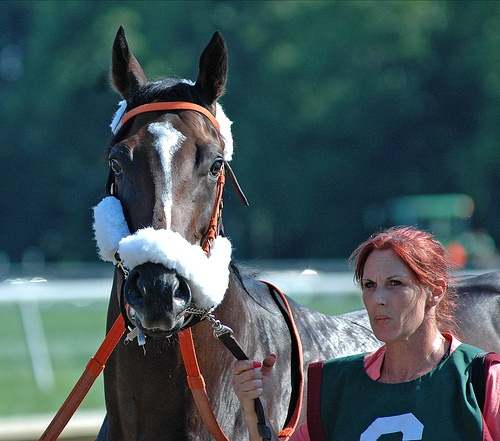
\includegraphics[width=.25\textwidth,height=.15\textwidth]{image/example/2007_000799.jpg}
		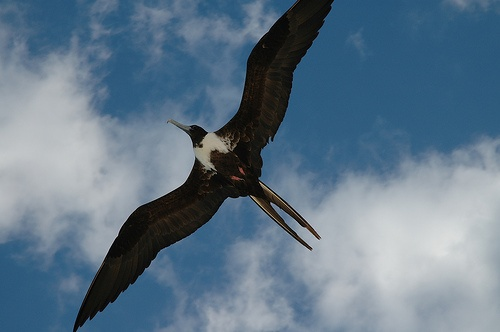
\includegraphics[width=.25\textwidth,height=.15\textwidth]{image/example/2007_002094.jpg}
		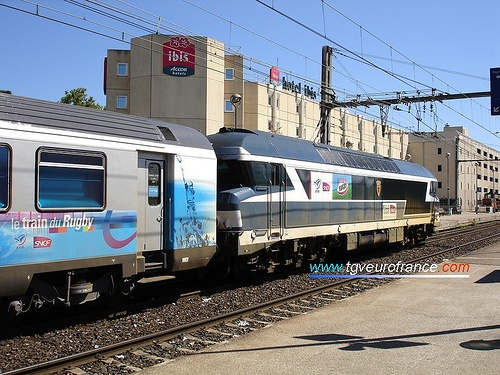
\includegraphics[width=.25\textwidth,height=.15\textwidth]{image/example/2007_004483.jpg}
		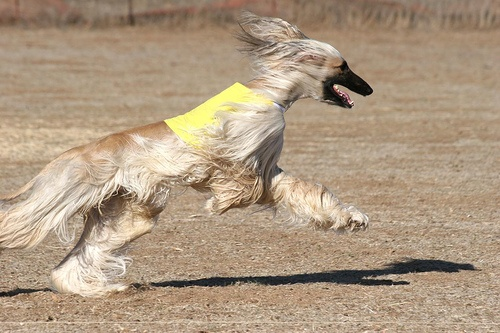
\includegraphics[width=.25\textwidth,height=.15\textwidth]{image/example/2007_003194.jpg}
		\caption{VOC 2012数据集:10582 张训练样本,1464张验证样本和1456张测试样本,21个类别}
	\end{figure}
	\vspace{-1.8em}
	\begin{figure}[h]
		\centering
		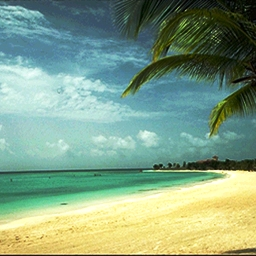
\includegraphics[width=0.25\textwidth,height=.15\textwidth]{figures/siftflow/coast_bea10.jpg}
		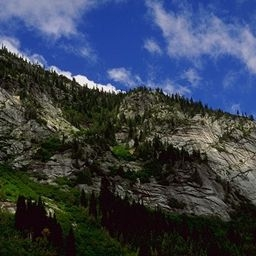
\includegraphics[width=0.25\textwidth,height=.15\textwidth]{figures/siftflow/mountain_n18058.jpg}
		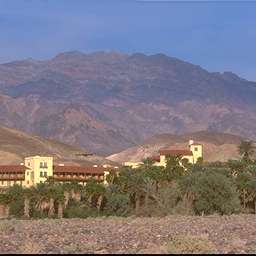
\includegraphics[width=0.25\textwidth,height=.15\textwidth]{figures/siftflow/opencountry_land732.jpg}
		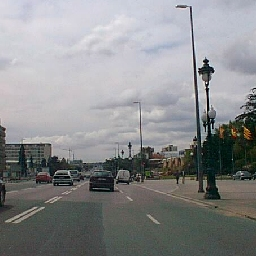
\includegraphics[width=0.25\textwidth,height=.15\textwidth]{figures/siftflow/highway_gre644.jpg}
		\caption{SIFT FLOW数据集:2488张训练样本,200张测试样本,33个类别}
		\label{fig:crop}
	\end{figure}
	\vspace{-1.2em}
	\footnotesize
	\begin{block}{图像预处理}
		\vspace{-0.5em}
		\begin{itemize}
			\item 训练时图像均缩放为321*321
			\item 随机选取训练图像,随机取镜像,数据白化
		\end{itemize}
	\end{block}
}

\frame{
	\frametitle{准确率度量方式}
	\begin{block}{}
		设$n_{ij}$为真实值属于类别$i$但被分类为类别$j$的像素个数,$n_{cl}$表示有多少种不同的标签,$t_i=\sum_{j=1}^{n_{cl}}n_{ij}$为所有真实值为类别$i$的像素个数。
		\begin{align}
			\begin{split}
				\mbox{像素准确率} &= \sum_{i=1}^{n_{cl}}n_{ii} / \sum_{i=1}^{n_{cl}}t_i \\
				\mbox{平均像素准确率} &= \frac{1}{n_{cl}} \sum_{i=1}^{n_{cl}}(n_{ii}/ t_i) \\
				\mbox{Mean IU} &= \frac{1}{n_{cl}} \sum_{i=1}^{n_{cl}}\frac{n_{ii}}{t_i + \sum_j^{n_{cl}} n_{ji} - n_{ii}}
			\end{split}
		\end{align}
	\end{block}
}
\subsection*{VOC 2012结果}
\frame{
	\frametitle{网格型长短记忆网络层数的选择}
	\begin{columns}
		\begin{column}{0.5\textwidth}
			\vspace{-0.8em}
			\begin{figure}
				\centering
				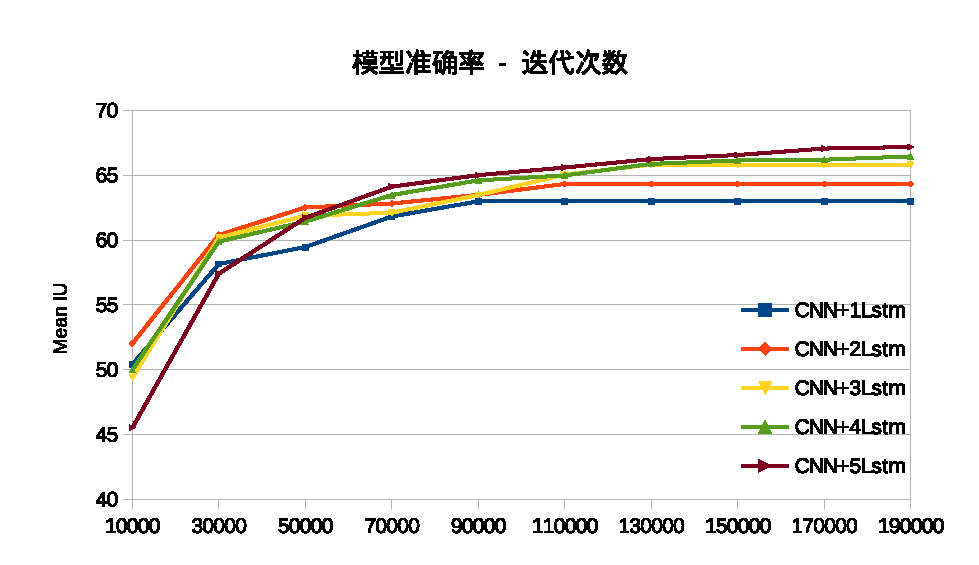
\includegraphics[width=\textwidth]{image/result/combine.eps}
				\caption{网格型长短记忆层数的不同对网络分割效果的影响方法}
				\label{fig:trainingaccuracy}
			\end{figure}
		\end{column}
		\vspace{-1.1em}
		\begin{column}{0.5\textwidth}
			\footnotesize
			\begin{itemize}
				\item[\dag] 在一定范围内增加长短记忆层数可以有效提高网络效果
				\item[\dag] 增加了5层网格型长短记忆网络之后,网络效果提升了\textbf{7.5\%}
			\end{itemize}
		\end{column}
	\end{columns}
	\vspace{-1em}
	\begin{figure}[h]
		\centering
		\makebox[0.11\textwidth]{\tiny 图像}
		\enspace
		\makebox[0.11\textwidth]{\tiny 真值}
		\enspace
		\makebox[0.11\textwidth]{\tiny CNN+5LSTM\textbf{1}}
		\enspace\thinspace
		\makebox[0.11\textwidth]{\tiny CNN+5LSTM\textbf{2}}
		\enspace\thinspace
		\makebox[0.11\textwidth]{\tiny CNN+5LSTM\textbf{3}}
		\enspace\thinspace
		\makebox[0.11\textwidth]{\tiny CNN+5LSTM\textbf{4}}
		\enspace\thinspace
		\makebox[0.11\textwidth]{\tiny CNN+5LSTM\textbf{5}}\\
		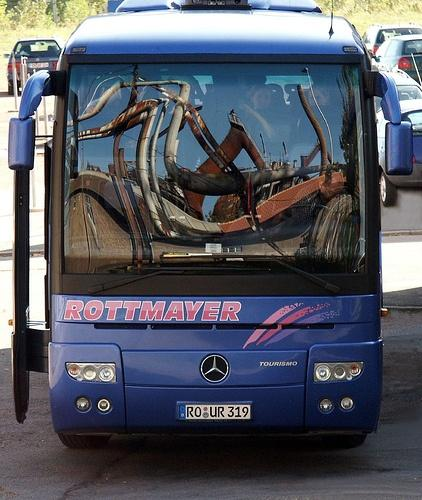
\includegraphics[width=0.11\textwidth]{image/improvement/2007_000663.jpg}
		\enspace\enspace %\hfill
		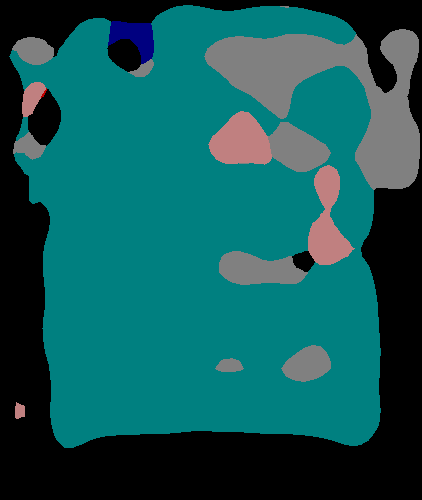
\includegraphics[width=0.11\textwidth]{image/improvement/2007_000663.png}
		\enspace\enspace
		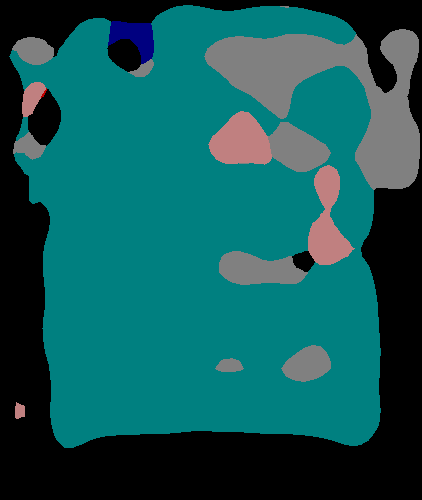
\includegraphics[width=0.11\textwidth]{image/improvement/2007_000663_1.png}
		\enspace\enspace
		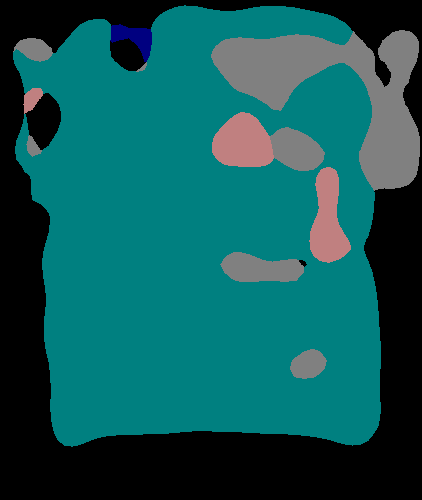
\includegraphics[width=0.11\textwidth]{image/improvement/2007_000663_2.png}
		\enspace\enspace
		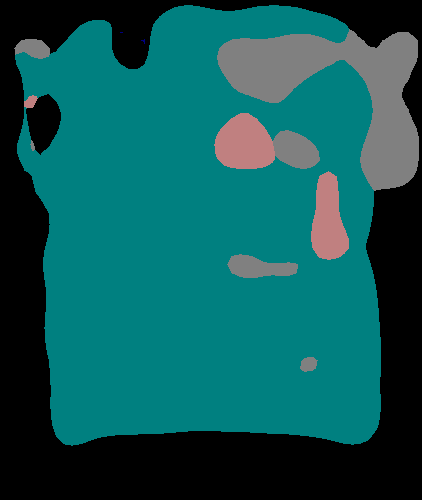
\includegraphics[width=0.11\textwidth]{image/improvement/2007_000663_3.png}
		\enspace\enspace
		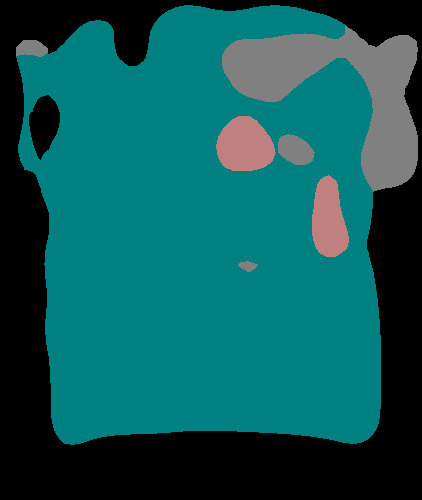
\includegraphics[width=0.11\textwidth]{image/improvement/2007_000663_4.png}
		\enspace\enspace
		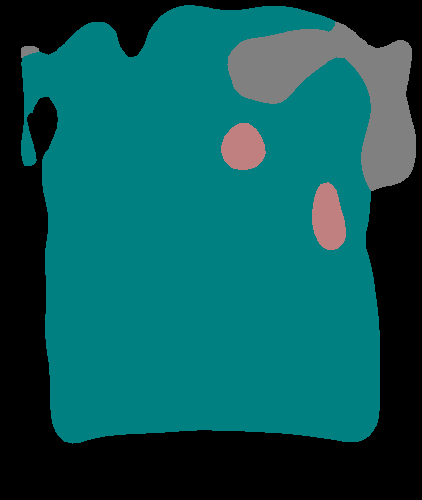
\includegraphics[width=0.11\textwidth]{image/improvement/2007_000663_5.png}
		\enspace\enspace
		\caption[同一网络网格型长短记忆网络时序的增加对输出改善作用的可视化]{网格型长短记忆网络层数增加对输出改善作用的可视化}
		\label{fig:improvement}
	\end{figure}
}

\frame{
	\frametitle{与其它工作的定量对比}
	\begin{table}[h] %voc table result
		\centering
		\resizebox{\textwidth}{!}{
			\begin{tabular}{c|*{20}{c}|c}
				\toprule
				Method                                                                                                             & aero          & bike          & bird          & boat          & bottle        & bus           & car           & cat           & chair         & cow           & table         & dog           & horse         & mbike         & person        & plant         & shep          & sofa          & train         & tv            & mIoU.         \\
				\midrule
				\midrule
				SDS\footnote{Simultaneous Detection and Segmentation, ECCV 2014}                                                   & 63.3          & 25.7          & 63.0          & 39.8          & 59.2          & 70.9          & 61.4          & 54.9          & 16.8          & 45.0          & 48.2          & 50.5          & 51.0          & 57.7          & 63.3          & 31.8          & 58.7          & 31.2          & 55.7          & 48.5          & 51.6          \\
				FCN-8s\footnote{Fully convolutional networks for semantic segmentation, CVPR 2015}                                 & 76.8          & 34.2          & 68.9          & 49.4          & 60.3          & 75.3          & 74.7          & 77.6          & 21.4          & 62.5          & 46.8          & 71.8          & 63.9          & 76.5          & 73.9          & 45.2          & 72.4          & 37.4          & 70.9          & 55.1          & 62.2          \\
				TTI-zoomout-16\footnote{Feedforward semantic segmentation with zoom-out features, CVPR 2015}                       & \textbf{81.9} & 35.1          & \textbf{78.2} & \textbf{57.4} & 56.5          & 80.5          & 74.0          & 79.8          & 22.4          & 69.6          & 53.7          & 74.0          & \textbf{76.0} & 76.6          & 68.8          & 44.3          & 70.2          & 40.2          & 68.9          & 55.3          & 64.4          \\
				DeepLab-CRF\footnote{Semantic image segmentation with deep convolutional nets and fully connected crfs, ICLR 2015} & 78.4          & 33.1          & \textbf{78.2} & 55.6          & \textbf{65.3} & 81.3          & 75.5          & 78.6          & \textbf{25.3} & 69.2          & 52.7          & \textbf{75.2} & 69.0          & \textbf{79.1} & \textbf{77.6} & \textbf{54.7} & 78.3          & 45.1          & 73.3          & 56.2          & 66.4          \\
				\midrule
				CNN+\textbf{5}LSTM                                                                                                 & 80.2          & \textbf{35.3} & 74.1          & 54.4          & 64.4          & \textbf{87.3} & \textbf{81.1} & \textbf{80.6} & 22.7          & \textbf{73.6} & \textbf{58.8} & 73.9          & 73.7          & 78.7          & 77.4          & 50.2          & \textbf{80.0} & \textbf{47.9} & \textbf{76.5} & \textbf{63.1} & \textbf{67.9} \\
				\bottomrule
			\end{tabular}}
		\caption[模型在VOC2012测试集上的结果]{模型在VOC2012测试集上的结果。}
		\label{tab:voctest}
	\end{table}
	\vspace{-1em}
	\begin{block}{结论}
		\begin{itemize}
			\item[\dag]模型比其他方法有更高的精确度,验证了模型的有效性
		\end{itemize}
	\end{block}
}
\frame{
	\frametitle{与其它工作的定性对比}
	\begin{figure} % image examples & compare
		\begin{subfigure}{0.55\textwidth}
			\centering
			\makebox[0.18\textwidth]{\tiny Grid-5LSTM}
			\makebox[0.18\textwidth]{\tiny FCN-8s}
			\makebox[0.18\textwidth]{\tiny SDS}
			\makebox[0.18\textwidth]{\tiny 真值}
			\makebox[0.18\textwidth]{\tiny 图像} \\
			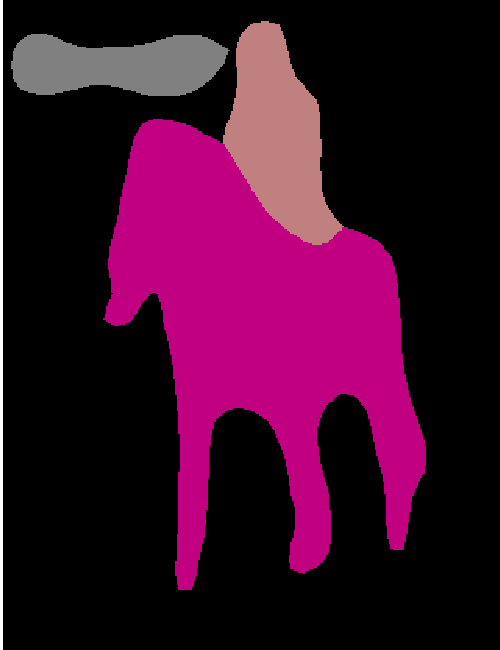
\includegraphics[width=0.18\textwidth]{image/result/compare/my_horse.pdf}
			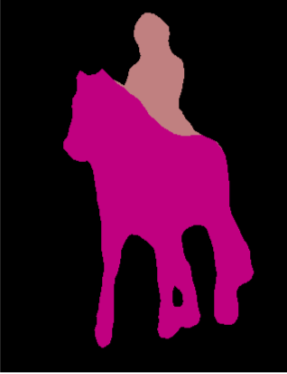
\includegraphics[width=0.18\textwidth]{image/result/compare/fcn_horse.png}
			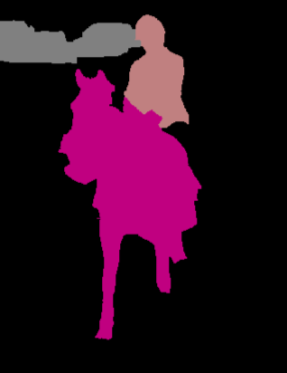
\includegraphics[width=0.18\textwidth]{image/result/compare/sds_horse.png}
			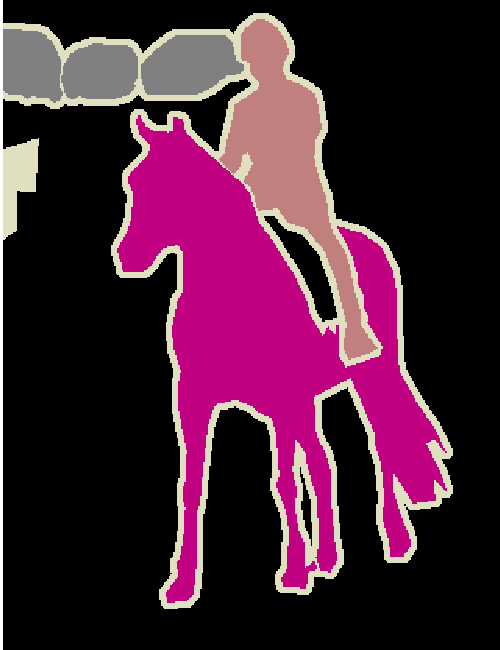
\includegraphics[width=0.18\textwidth]{image/result/compare/gt_horse.pdf}
			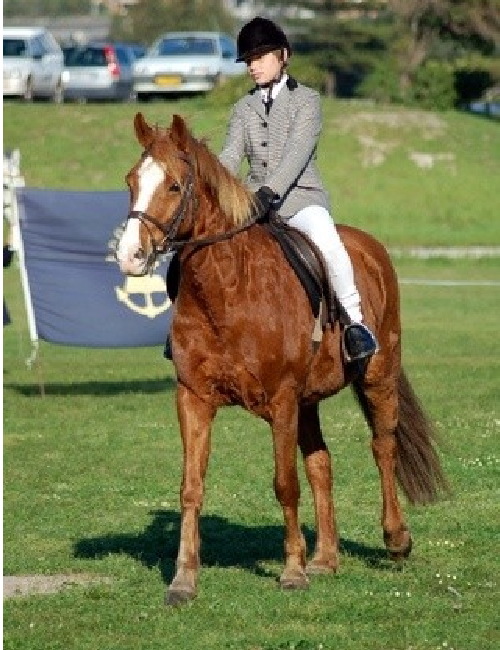
\includegraphics[width=0.18\textwidth]{image/result/compare/im_horse.pdf}
			\\
			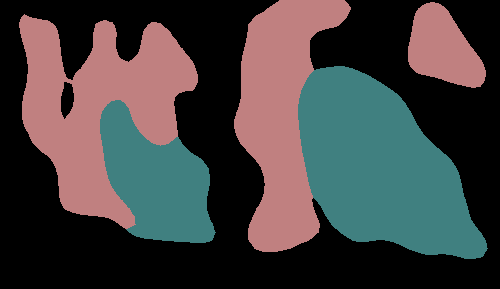
\includegraphics[width=0.18\textwidth]{image/result/compare/my_motor.png}
			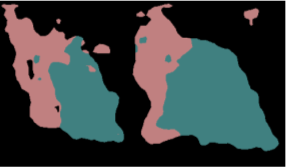
\includegraphics[width=0.18\textwidth]{image/result/compare/fcn_motor.png}
			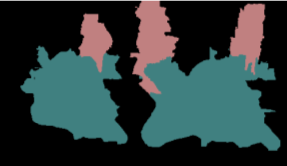
\includegraphics[width=0.18\textwidth]{image/result/compare/sds_motor.png}
			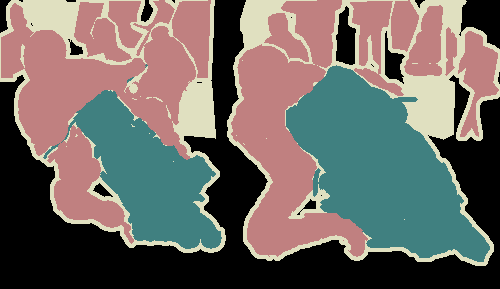
\includegraphics[width=0.18\textwidth]{image/result/compare/2007_005173.png}
			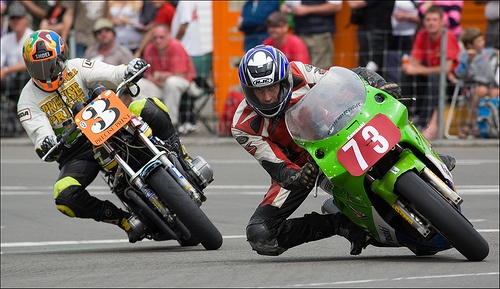
\includegraphics[width=0.18\textwidth]{image/result/compare/2007_005173.jpg}
			\\
			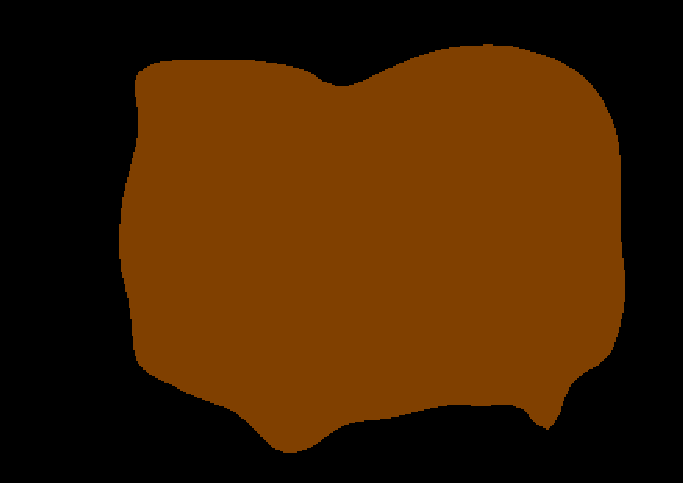
\includegraphics[width=0.18\textwidth]{image/result/compare/my_sheep.pdf}
			
\includegraphics[width=0.18\textwidth]{image/result/compare/fcn_sheep.png}
			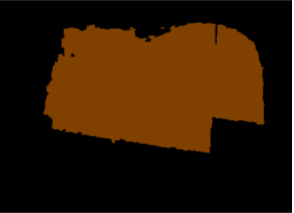
\includegraphics[width=0.18\textwidth]{image/result/compare/sds_sheep.png}
			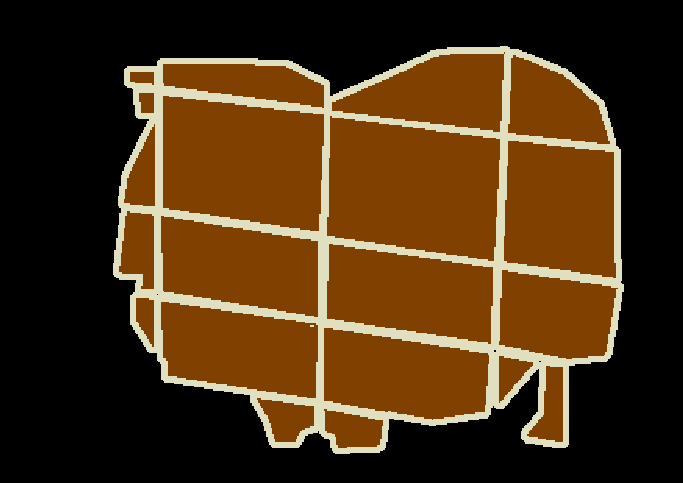
\includegraphics[width=0.18\textwidth]{image/result/compare/gt_sheep.pdf}
			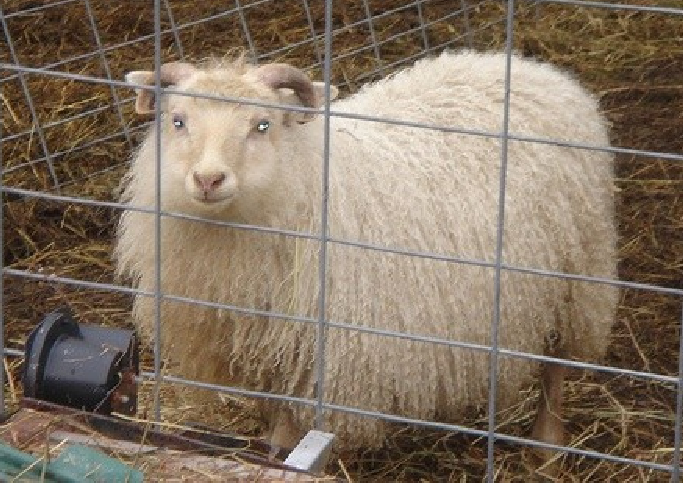
\includegraphics[width=0.18\textwidth]{image/result/compare/im_sheep.pdf}
			\\
			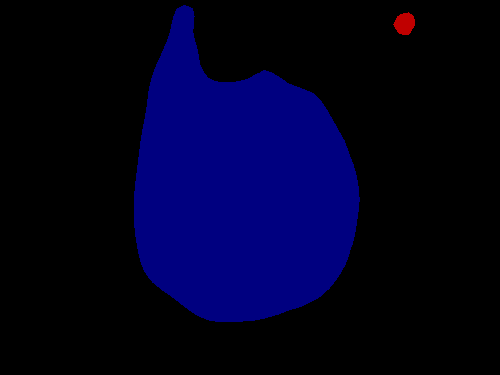
\includegraphics[width=0.18\textwidth]{image/result/compare/my_boat.png}
			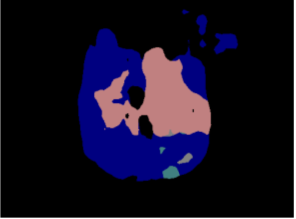
\includegraphics[width=0.18\textwidth]{image/result/compare/fcn_boat.png}
			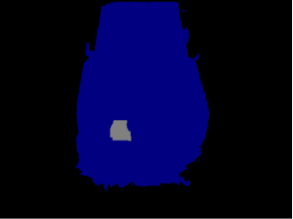
\includegraphics[width=0.18\textwidth]{image/result/compare/sds_boat.png}
			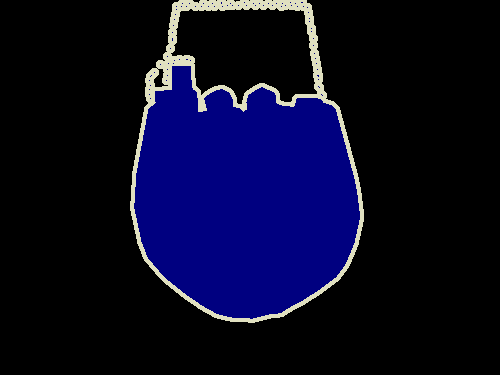
\includegraphics[width=0.18\textwidth]{image/result/compare/2007_004241.png}
			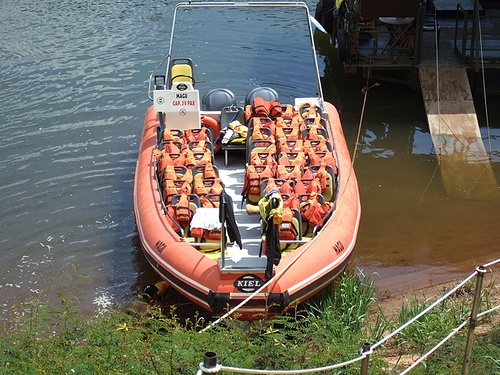
\includegraphics[width=0.18\textwidth]{image/result/compare/2007_004241.jpg}
			\caption{本文模型效果与其他工作的定性对比}
			\label{fig:compare1}
		\end{subfigure}
		\begin{subfigure}{0.4\textwidth}
			\centering

			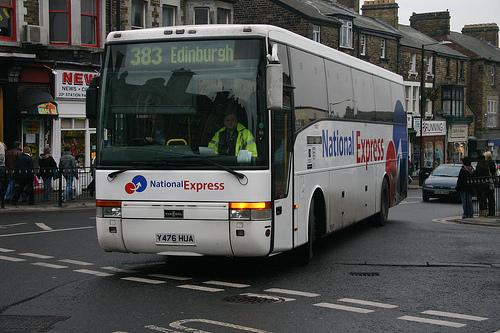
\includegraphics[width=0.25\textwidth]{image/result/compare/2010_005284.jpg}
			\includegraphics[width=0.25\textwidth]{image/result/compare/2007_003349.jpg}
			\includegraphics[width=0.25\textwidth]{image/result/compare/2009_004507.jpg}
			\\
			\includegraphics[width=0.25\textwidth]{image/result/compare/2010_005284.png}
			\includegraphics[width=0.25\textwidth]{image/result/compare/2007_003349.png}
			\includegraphics[width=0.25\textwidth]{image/result/compare/2009_004507.png} \\
			\includegraphics[width=0.25\textwidth]{image/result/compare/zoom_bus.png}
			\includegraphics[width=0.25\textwidth]{image/result/compare/zoom_bird.png}
			\includegraphics[width=0.25\textwidth]{image/result/compare/zoom_dog.png} \\
			\includegraphics[width=0.25\textwidth]{image/result/compare/deeplab_bus.png}
			\includegraphics[width=0.25\textwidth]{image/result/compare/deeplab_bird.png}
			\includegraphics[width=0.25\textwidth]{image/result/compare/deeplab_dog.png} \\
			\includegraphics[width=0.25\textwidth]{image/result/compare/my_bus.png}
			\includegraphics[width=0.25\textwidth]{image/result/compare/my_bird.png}
			\includegraphics[width=0.25\textwidth]{image/result/compare/my_dog.png}
			\caption{\tiny 其中第一行为图像,第二行为真值,第三行为TTI-zoomout-16,第四行为DeepLab-CRF,第五行是Grid-5LSTM的结果}
			\label{fig:compare2}
		\end{subfigure}
		\caption{Grid-5LSTM与其它模型在VOC 2012验证集上的定性比较}
	\end{figure}
}

\frame{
	\frametitle{一些分割失败的例子}
	\begin{figure}[h]
		\centering
		\makebox[0.15\textwidth]{\footnotesize 图像}
		\makebox[0.15\textwidth]{\footnotesize 真值}
		\makebox[0.15\textwidth]{\tiny CNN+5LSTM}
		\quad
		\makebox[0.15\textwidth]{\footnotesize 图像}
		\makebox[0.15\textwidth]{\footnotesize 真值}
		\makebox[0.15\textwidth]{\tiny CNN+5LSTM}\\
		\includegraphics[width=0.15\textwidth]{image/result/error/2008_000673.jpg}
		\includegraphics[width=0.15\textwidth]{image/result/error/2008_000673.png}
		\includegraphics[width=0.15\textwidth]{image/result/error/p_2008_000673.png}
		\quad
		\includegraphics[width=0.15\textwidth]{image/result/error/2008_001580.jpg}
		\includegraphics[width=0.15\textwidth]{image/result/error/2008_001580.png}
		\includegraphics[width=0.15\textwidth]{image/result/error/p_2008_001580.png}
		\\
		\includegraphics[width=0.15\textwidth]{image/result/error/2007_002539.jpg}
		\includegraphics[width=0.15\textwidth]{image/result/error/2007_002539.png}
		\includegraphics[width=0.15\textwidth]{image/result/error/p_2007_002539.png}
		\quad
		\includegraphics[width=0.15\textwidth]{image/result/error/2007_008964.jpg}
		\includegraphics[width=0.15\textwidth]{image/result/error/2007_008964.png}
		\includegraphics[width=0.15\textwidth]{image/result/error/p_2007_008964.png}
		\\
		\includegraphics[width=0.15\textwidth]{image/result/error/2008_000763.jpg}
		\includegraphics[width=0.15\textwidth]{image/result/error/2008_000763.png}
		\includegraphics[width=0.15\textwidth]{image/result/error/p_2008_000763.png}
		\quad
		\includegraphics[width=0.15\textwidth]{image/result/error/2007_009088.jpg}
		\includegraphics[width=0.15\textwidth]{image/result/error/2007_009088.png}
		\includegraphics[width=0.15\textwidth]{image/result/error/p_2007_009088.png}
		\\
		\color[rgb]{0.9,0.9,0.9}\bfseries
		\resizebox{\textwidth}{!}{
			\begin{tabular}{*{7}{>{\centering\arraybackslash}p{0.111\textwidth}}}
				\hline
				\cellcolor[rgb]{0,0,0}  背景                 & \cellcolor[rgb]{0.5020,0,0} 飞机         & \cellcolor[rgb]{0,0.5020,0} 自行车 & \cellcolor[rgb]{0.5020,0.5020,0} 鸟 & \cellcolor[rgb]{0,0,0.5020} 船        & \cellcolor[rgb]{0.5020,0,0.5020} 瓶子 & \cellcolor[rgb]{0,0.5020,0.5020} 大巴
				\\
				\hline
				\cellcolor[rgb]{0.5020,0.5020,0.5020} 汽车   & \cellcolor[rgb]{0.2510,0,0} 猫           & \cellcolor[rgb]{0.7529,0,0} 椅子   & \cellcolor[rgb]{0.2510,0.5020,0} 牛 & \cellcolor[rgb]{0.7529,0.5020,0} 桌子 & \cellcolor[rgb]{0.2510,0,0.5020} 狗   & \cellcolor[rgb]{0.7529,0,0.5020} 马   \\
				\hline
				\cellcolor[rgb]{0.2510,0.5020,0.5020} 摩托车 & \cellcolor[rgb]{0.7529,0.5020,0.5020} 人 & \cellcolor[rgb]{0,0.2510,0} 盆栽   & \cellcolor[rgb]{0.5020,0.2510,0} 羊 & \cellcolor[rgb]{0,0.7529,0} 沙发      & \cellcolor[rgb]{0.5020,0.7529,0} 火车 & \cellcolor[rgb]{0,0.2510,0.5020} 电视 \\
				\hline
			\end{tabular}
		}
		\caption[一些模型分类错误的例子]{一些CNN+5LSTM分类错误的例子}
		\label{fig:error}
	\end{figure}
}

\subsection*{SIFT FLOW实验结果}
\frame{
	\frametitle{SIFT FLOW实验结果}
	\begin{table}[h] %voc table result
		\centering
		\resizebox{0.8\textwidth}{!}{
			\begin{tabular}{*{4}{c}}
				\toprule
				Method                                                                                                                 & Pixel Acc.    & Mean Acc.     & Mean IU.      \\
				\midrule
				Liu et al.\footnote{Sift flow: Dense correspondence across scenes and its applications, PAMI 2011}                     & 76.7          & -             & -             \\
				Tighe et al.\footnote{Finding things: Image parsing with regions and per-exemplar detectors, CVPR 2013}                & 78.6          & 39.2          & -             \\
				FCN-16s\footnote{Fully convolutional networks for semantic segmentation, CVPR 2015}                                    & 85.2          & \textbf{51.7} & 39.5          \\
				Deeplab-LargeFOV\footnote{emantic image segmentation with deep convolutional nets and fully connected crfs, ICLR 2015} & 85.6          & 51.2          & 39.7          \\
				\midrule
				Grid-5LSTM                                                                                                             & \textbf{86.2} & 51.0          & \textbf{41.2} \\
				\bottomrule
			\end{tabular}
		}
		\caption[模型在SIFT FLOW上的结果]{模型在SIFT FLOW上的结果。Tighe等人的方法是用SVM+MRF,Deeplab-LargeFOV的结果是通过公开的源码实验得到的}
		\label{tab:siftflow}
	\end{table}
}

\endinput

% \chapter{总结与展望}

\label{cha:conclusion}

本文提出了一个新的UDA框架用于跨模态医学图像分割。该框架利用解耦表示学习来提取多模态图像的解剖学特征和模态特征,同时利用对抗学习来进行图像自适应和特征自适应的融合。我们在不成对的多模态心脏数据集MMWHS上验证了该方法的效果。实验结果表明该框架改进域位移问题的有效性。

对于未来的工作,可以把该框架从2D图像扩展到与临床诊断更相关的3D图像,同时应用到不同的多模态数据集上来验证方法的鲁棒性以及泛化性,此外,可以利用生成对抗网络来进行多模态医学图像的生成进行自监督训练来缓解缺乏带标注医学图像数据的问题。

% \section{致谢}
\subsection*{致谢}
\frame{
	\frametitle{致谢}
	\begin{block}{感谢每一个帮助过我的人}
		\begin{itemize}
			\item 首先要感谢的是我的指导老师的悉心指导
			\item 感谢师兄师姐、同学的帮助
			\item 感谢家人的支持
			\item 感谢答辩委员会的聆听和指导
		\end{itemize}
	\end{block}
	\vspace{-1em}
	\note{
		我的展示到此结束,我要感谢我的指导老师,师兄师姐同学,家人还有答辩委员会老师的聆听与指导。谢谢大家
	}
}
\frame{
	\frametitle{Q \& A}
	\begin{block}{Questions?}
		~\\ ~\\
		\center{\Large{Thank you!}}
		\\ ~\\ ~\\ ~\\ ~\\
	\end{block}
	\note{
		现在是问答时间。请问老师们对我的展示有什么疑问?
	}
}



\end{document}
